\documentclass[12pt,titlepage]{book}
\usepackage[margin=0.9in]{geometry} 
\usepackage{amsmath,amsthm,amssymb,graphicx,mathtools,tikz,hyperref}
\usepackage{pgfplots}
\usepackage{xcolor}
\newcommand{\redp}[1]{\textcolor{red}{#1}}
\newcommand{\bluep}[1]{\textcolor{blue}{#1}}
\newcommand{\tealp}[1]{\textcolor{teal}{#1}}
\usepackage{tcolorbox}
\newtcolorbox{mybox}{colback=red!5!white,colframe=red!75!black,fonttitle=\bfseries,title=Box}
\newtcolorbox{qt}{colback=orange!5!white,colframe=orange!75!white}
\usetikzlibrary{patterns,hobby}
\numberwithin{equation}{section}
\usepackage{wrapfig}
\usepackage{indentfirst}
\usepackage{ragged2e}
\RaggedRightParindent = 24 pt
\setlength{\parskip}{0.8em}
\renewcommand{\baselinestretch}{1.5}
\usepackage[noline]{algorithm2e}
\SetAlFnt{\footnotesize}
\usepackage{graphicx}
\usepackage{titling}
\renewcommand\maketitlehooka{\null\mbox{}\vfill}
\renewcommand\maketitlehookd{\vfill\null}
\usepackage{tocloft}
\renewcommand\cftsecafterpnum{\vskip6pt}
\usepackage{makeidx}
\makeindex
\usepackage{mdframed}
\newenvironment{que}
    { \begin{mdframed}[backgroundcolor=green!20] \textbf{$\Delta$ Question} \\}
    {  \end{mdframed}}
\newenvironment{thm}
    { \begin{mdframed}[backgroundcolor=orange!20] \textbf{$\Delta$ Theorem} \\}
    {  \end{mdframed}}
\newenvironment{defi}
    { \begin{mdframed}[backgroundcolor=red!10] \textbf{$\Delta$ Definition} \\}
    {  \end{mdframed}}
\newenvironment{lemma}
    { \begin{mdframed}[backgroundcolor=gray!10] \textbf{$\cdot$ Lemma} \\}
    {  \end{mdframed}}
\newenvironment{example}
    { \begin{mdframed}[backgroundcolor=white!10] \textbf{$\cdot$ Example} \\}
    {  \end{mdframed}}
\usepackage{graphicx}
\usepackage{float}
\usepackage{longtable}
\usepackage{tikz}
\usepackage{esint}
\usepackage{CJKutf8}

\title{Quantum Field Theory for Educated Dummies}
\author{Sizhe Liu\\University of Illinois at Urbana-Champaign }
\date{Version 1.0}

\pgfplotsset{compat=1.15}

\begin{document}

\maketitle

\chapter{Foundations}
\section{Natural Units and Dimensions}
Convenient systems of units start with arbitrary definitions for units of certain fundamental. quantities and derive the remaining units from laws of nature. To see how this works, assume we know three basic laws of nature and we want to devise a system of units from scratch. We will do this first for the cgs system and then for natural units.
The three lawas are:
\begin{qt}
\begin{itemize}
    \item The distance $L$ traveled by a photon is the speed of light multiplied by its time of travel. $L=c t$
    \item The energy of a massive particle is equal to its mass (at rest) $m$ times the speed of light squared. $E=mc^2$
    \item The energy of a photon is proportional to its frequency $f$. The constant of proportionality is Planck's constant $h . E=h f$ or re-expressed as $E=\hbar \omega$
\end{itemize}
\end{qt}
In natural units:\redp{the $c$ and $\hbar$ are dimensionless and equal to 1. The unit for energy is $MeV$}.

\section{Notation}
We shall use a notation defining \textbf{contravariant components $x^{\mu}$ of the $4 \mathrm{D}$ position vector} as $3 \mathrm{D}$ Cartesian coordinates $X_{i}$ plus $c t$ (see Appendix $\bar{A}$ if you are not comfortable with this), i.e.,
\begin{equation}
x^{\mu}=\left[\begin{array}{l}
{x^{0}} \\
{x^{1}} \\
{x^{2}} \\
{x^{3}}
\end{array}\right]=\left[\begin{array}{l}
{c t} \\
{X_{1}} \\
{X_{2}} \\
{X_{3}}
\end{array}\right]=\left[\begin{array}{l}
{c t, X_{i}}
\end{array}\right]^{T}
\end{equation}
From special relativity, we know the differential proper time passed on an object (with $c=1$ ) is
\begin{equation}
(d \tau)^{2}=(d t)^{2}-d X_{1} d X_{1}-d X_{2} d X_{2}-d X_{3} d X_{3}
\end{equation}
If we define \textbf{covariant components} of the 4D position vector as
\begin{equation}
x_{\mu}=\left[\begin{array}{l}
{x_{0}} \\
{x_{1}} \\
{x_{2}} \\
{x_{3}}
\end{array}\right]=\left[\begin{array}{c}
{t} \\
{-X_{1}} \\
{-X_{2}} \\
{-X_{3}}
\end{array}\right]=\left[t,-X_{i}\right]^{T}
\end{equation}
then
\begin{equation}
(d \tau)^{2}=d x^{0} d x_{0}+d x^{1} d x_{1}+d x^{2} d x_{2}+d x^{3} d x_{3}=d x^{\mu} d x_{\mu}
\end{equation}
Using metric tensor $g_{\mu\nu}$, we have the following relation:
\begin{equation}
x_{\mu}=g_{\mu \nu} x^{\nu}=\left[\begin{array}{cccc}
{1} & {0} & {0} & {0} \\
{0} & {-1} & {0} & {0} \\
{0} & {0} & {-1} & {0} \\
{0} & {0} & {0} & {-1}
\end{array}\right]\left[\begin{array}{c}
{x^{0}} \\
{x^{1}} \\
{x^{2}} \\
{x^{3}}
\end{array}\right]
\end{equation}
\redp{The inverse of $g_{\mu\nu}$, $g^{\mu\nu}$, has the exact same form.}Thus,
\begin{equation}
(d \tau)^{2}=g_{\mu v} d x^{\mu} d x^{v}=g^{\mu v} d x_{\mu} d x_{v}
\end{equation}
\begin{qt}
Partial derivative w.r.t. $x^{\mu}$ and $x_{\mu}$ are:
\begin{equation}
\partial_{\mu}=\frac{\partial}{\partial x^{\mu}}=\left(\frac{\partial}{\partial t}, \frac{\partial}{\partial x^{i}}\right)^{T}=\left(\frac{\partial}{\partial t} \cdot \frac{\partial}{\partial X_{i}}\right)^{T}
\end{equation}
and
\begin{equation}
\partial^{\mu}=\frac{\partial}{\partial x_{\mu}}=\left(\frac{\partial}{\partial t}, \frac{\partial}{\partial x_{i}}\right)^{T}=\left(\frac{\partial}{\partial t},-\frac{\partial}{\partial X_{i}}\right)^{T}
\end{equation}
\end{qt}
For a matrix, we can raise the index as
\begin{equation}
M^{\mu \nu}=g^{\mu \alpha} g^{\nu \beta} M_{\alpha \beta}
\end{equation}
\section{Review of Variational Methods}
Recall also, that given the Lagrangian, we could find the Hamiltonian $H,$ via the Legendre transformation (employing a Cartesian system where $x^{i}=x_{i}$ and $p^{i}=p_{i}$),
\begin{equation}
H=p_{i} \dot{x}^{i}-L, \quad \text { where } p_{i}=\frac{\partial L}{\partial \dot{x}^{i}}=m \dot{x}^{i}\left(=p^{\prime} \text { for Cartesian system }\right)
\end{equation}
$p_{i}$ is the conjugate, or canonical, momentum of $x$ '. (Note that a contravariant component in the denominator is effectively equivalent to a covariant component in the entire entity, and vice versa.) Hence, we can define:
\begin{qt}
\textbf{First quantization}

Keeping the classical Hamiltonian and, changing Poisson brackets to commutators, we could just as readily have used the Lagrangian L, or the equations of motion instead.
\end{qt}
\subsection{Classical Field Theory}
From particle theory to field theory, we have the following things changed:
\begin{qt}
$$L, H, e t c \rightarrow \mathcal{L}, \mathcal{H},$$ 
\[
x^{i}(t) \rightarrow \phi^{r}\left(x^{\mu}\right)
\]
$$t \rightarrow x^{\mu}$$
\end{qt}
Classical field theory is analogous in many ways to classical particle Lagrangian $L$, we have the Lagrangian density $\mathcal{L}$. Instead of time $t$ as an independent variable, we have $x^{\mu}=x^{0}, x^{1}, x^{2}, x^{3}=t, {x^{i}}$ as independent variables. Instead of a particle described by $x^{i}(t),$ \textbf{we have a field value described by $\phi(x^{\mu})$, where $r$ designates different field types, or possibly, different spatial components of the same vector field.}
\begin{qt}
The Euler-Lagrange equation for fields becomes
\begin{equation}
\frac{\partial}{\partial x^{\mu}}\left(\frac{\partial \mathcal{L}}{\partial \phi^{r}, \mu}\right)-\frac{\partial \mathcal{L}}{\partial \phi^{r}}=0
\end{equation}
and
\begin{equation}
\mathcal{H}=\pi_{r} \dot{\phi}^{r}-\mathcal{L}, \quad \text { where } \pi_{r}=\frac{\partial \mathcal{L}}{\partial \dot{\phi}^{r}}
\end{equation}
with $\pi_r$ being the conjugate momentum density of the field $\phi^r$. And the action is
\begin{equation}
S=\int_{T} \int_{V} \mathcal{L}\left(\phi, \phi_{,\mu}\right) d^{3} \mathbf{x} d t=\int_{\Omega} \mathcal{L}\left(\phi, \phi_{, \mu}\right) d^{4} x
\end{equation}
\end{qt}
\subsection{Key concepts in field theory}
For fields
\begin{equation}
\frac{\partial \phi}{\partial t}=\frac{d \phi}{d t}=\dot{\phi}
\end{equation}
This is generally not true for other quantities. For fields, 
\begin{equation}
\frac{d \phi}{d t}=\frac{\partial \phi}{\partial x^{\prime}} \frac{d x^{\prime}}{d t}+\frac{\partial \phi}{\partial t} \frac{d t}{d t}
\end{equation}
\redp{where $\frac{dx^i}{dt}$ are equal to zero}.

For a single particle, particle position coordinates are the generalized coordinates and particle momentum components are its conjugate momenta. For fields, each field is itself a generalized coordinate and each field has its own conjugate momentum (density). As noted, this field conjugate momentum (density) is different from the physical momentum (density) that the field possesses.

For conjugate and physical momentum densities, we have the following density relation
$$
p_{t}=\frac{\partial L}{\partial \dot{x}^{t}} \quad \frac{\text { for small particle in medium, }}{\text { divide by particle volume }}, \quad \mathcal{R}_{i}=\frac{\partial \mathcal{L}}{\partial \dot{x}^{i}}
$$
We note carefully that our $x^i$ here is the position coordinate of a point fixed relative to the field and thus is time dependent. Further, the total derivative $\dot{x}^i$ equals the partial derivative w.r.t. time, since $x^i$ in the present case is only a function of time. Now take the \redp{conjugate momentum density relation for relativistic fields},
$$
\pi_{r}=\frac{\partial \mathcal{L}}{\partial \dot{\phi}^{r}}
$$
and
$$
\frac{\mathcal{R}_{i}}{\pi_{r}}=\frac{\partial \mathcal{L} / \partial \dot{x}^{i}}{\partial \mathcal{L} / \partial \dot{\phi}^{r}}=\frac{\partial \dot{\phi}^{r}}{\partial \dot{x}^{\prime}}=\frac{\partial \phi^{r} / \partial t}{\partial x^{i} / \partial t}=\frac{\partial \phi^{r}}{\partial x^{i}} \quad \rightarrow \quad \mathcal{R}_{i}=\pi_{r} \frac{\partial \phi^{r}}{\partial x^{i}} \quad \rightarrow \quad \mathcal{R}^{i}=-\pi_{r} \frac{\partial \phi^{r}}{\partial x^{i}}
$$
The partial derivative of $\phi^{r}$ with respect to either of our definitions of $x^{i}$ (time dependent as the moving position of a point fixed to the field, or time independent as coordinates fixed in space) is the same because by definition, partial derivative means we hold everything else here constant, Thus, the above relation holds in field theory when we consider the $x^{i}$ as independent variables (coordinates fixed in space).

The field equation (equations of motion) for relativistic fields keep the exact same form in any inertial frame of reference, i.e., they are \redp{Lorentz invariant}. Four scalars(world scalars) are \redp{invariant under a Lorentz transformation and look exactly the same to any observer.}
\begin{qt}
The mass $m$ in relativity of a free particle is four scalar, where $m^2=p^{\mu}p_{\mu}$.

Demanding that the Euler-Lagrange equation be Lorentz invariant, we know that, within that equation, $x^{\mu}$,$\phi^r$, and derivatives of $x^{\mu}$ are Lorentz covariant or invariant. \redp{So, in order for the whole equation to be Lorentz invariant, the Lagrangian density $\mathcal{L}$ must be invariant.}

Further, L, H, and $\mathcal{H}$ are not Lorentz scalars.
\end{qt}

\section{Schrodinger vs. Heisenberg Pictures}
In Schrodinger picture, the expectation value is calculated as:
$$
\overline{\mathcal{O}}=\int \psi^{\dagger} \mathcal{O} \psi d^{3} x=\langle\psi|\mathcal{O}| \psi\rangle
$$
The time derivative of the expectation value is
\begin{equation}
\frac{d \bar{\mathcal{O}}}{d t}=\frac{d}{d t}\langle\psi|\mathcal{O}| \psi\rangle=\left\langle\frac{\partial \psi}{\partial t}|\mathcal{O}| \psi\right\rangle+\left\langle\psi\left|\frac{\partial \mathcal{O}}{\partial t}\right| \psi\right\rangle+\left\langle\psi|\mathcal{O}| \frac{\partial \psi}{\partial t}\right\rangle
\end{equation}
where we use partial derivative in the brackets because our states and operators are functions of $x^i$ and $t$.

In the Schródinger picture (S.P.), the solutions to the Schrödinger equation

\begin{equation}
i \frac{\partial \psi_{S}}{\partial t}=H \psi_{S} \quad \text { or } \quad i \frac{\partial}{\partial t}|\psi\rangle_{S}=H|\psi\rangle_{S}
\label{schrodinger-equation}
\end{equation}
\redp{In the Schrodinger picture, the operators are usually not time dependent.} For example, using the familiar momentum operator $p_1^S=i\partial/\partial x^1$ for the S.P. in the $x^1$ direction, with 
$$
\psi_{S}=A e^{-i\left(E t-p\cdot x\right)}=|\psi\rangle_{S} \quad A^{\dagger} A=\frac{1}{V}
$$
we have
$$
\begin{array}{l}
{\bar{p}_{1}=\int A^{+} e^{i\left( Et-p^{\prime}x^{\prime}\right)}\left(i \frac{\partial}{\partial x^{1}}\right) A e^{-i\left(Et-p^{\prime}x^{\prime}\right)} d^{3} x={}_{s}\langle\psi|p_{1}^{S}| \psi\rangle_{s}}
\end{array}
$$
Since there is no $t$ in the operator, we have
$$
\frac{d p_{1}^{S}}{d t}=\frac{\partial p_{1}^{S}}{\partial t}=0
$$
and
\begin{equation}
\frac{d \bar{p}_{1}}{d t}=\frac{d}{d t}\left\langle\psi\left|p_{1}^{s}\right| \psi\right\rangle=\left\langle\frac{\partial \psi}{\partial t}\left|p_{1}^{s}\right| \psi\right\rangle_{s}+s\left\langle\psi\left|\frac{\partial p_{1}^{s}}{\partial t}\right| \psi\right\rangle_{s}+s\left\langle\psi\left|p_{1}^{s}\right| \frac{\partial \psi}{\partial t}\right\rangle_{s}
\end{equation}
Using (\ref{schrodinger-equation}), and its complex conjugate, we have
\begin{equation}
\frac{d \bar{p}_{1}}{d t}=_{S}\left\langle\psi\left|\left(i H p_{1}^{S}+\frac{\partial p_{1}^{S}}{\partial t}-i p_{1}^{S} H\right)\right| \psi\right\rangle_{S}=_{S}\left\langle\psi\left|-i\left[p_{1}^{S}, H\right]\right| \psi\right\rangle_{S}+_{S}\left\langle\psi\left|\frac{\partial p_{1}^{S}}{\partial t}\right| \psi\right\rangle_{S}
\end{equation}
where the last term is equal to zero.\redp{Recall the old NRQM adage that the expectation value of any operator without explicit time dependence that commutes with the Hamiltonian is conserved (its time derivative is zero.)}

\textbf{\redp{The Schrodinger picture states and operators can be transformed to states and operators having different form via what is known as a unitary transformation. The particular unitary transformation (where $U$ is a unitary operator) for this is}}
\begin{qt}
\begin{equation}
U=e^{-i A t} \quad\left(=e^{-i H t / \hbar} \text { in non-natural units }\right)
\end{equation}
where states and operators transform as
\begin{equation}
\begin{array}{ll}
{U^{\dagger}|\psi\rangle_{S}=|\psi\rangle_{H}} & {U^{\dagger} \mathcal{O}^{S} U=\mathcal{O}^{H}} \\
{U|\psi\rangle_{H}=|\psi\rangle_{S}} & {U O^{H} U^{\dagger}=\mathcal{O}^{S}}
\end{array}
\end{equation}
\end{qt}
We find that in the first relation the state is now \redp{time independent} in H.P. 

Taking the time derivative in the second relation, we have:
\begin{equation}
\begin{aligned}
\frac{d}{d t}\left(U^{\dagger} \mathcal{O}^{S} U\right) &=(i H) \underbrace{e^{i A^{\prime}} \mathcal{O}^{S}}_{\mathcal{O}^{H}}+\underbrace{e^{i H_{t}}\left(\frac{\partial \mathcal{O}^{S}}{\partial t}\right) e^{-i H_{l}}}_{\text {defined as } \hat{\partial} O^{H} / \partial t}+\underbrace{e^{i H t} \mathcal{O}^{S} e^{-t H t}}_{\mathcal{O}^{H}}(-i H) \\
&=\frac{d \mathcal{O}^{H}}{d t}=-i\left[\mathcal{O}^{H}, H\right]+\frac{\hat{\partial} \mathcal{O}^{H}}{\partial t}
\end{aligned}
\end{equation}
In this note, $\frac{\hat{\partial} \mathcal{O}^{H}}{\partial t}$ will always be zero. Nonetheless, we see that in the H.P., an operator time derivative can be \textbf{non-zero},\redp{and the operator is time dependent}.
\begin{mybox}
A unitary transformation is called unitary because its operation on (transformation of ) a state vector leaves the magnitude of the state vector unchanged, i.e., the state vector magnitude is multiplied by unity.

A unitary transformation can be thought of as "rotating" a (complex number) state vector in Hilbert space (the complex space where each coordinate axis is an eigenvector) without changing the "length".

Recall, from classical mechanics, that an orthogonal transformation represented by a real matrix $\mathbf{A}$ has an inverse equal to the transpose of that matrix, i.e., $\mathrm{A}^{-1}=\mathrm{A}^{\mathrm{T}}$. In the complex space of state vectors, a unitary transformation $U$ has an analogous form for its inverse, the complex conjugate transpose, i.e., $\underline{U}^{-1}=U^{+}$ and so $U^{\dagger} U=1 .$ The following example may make this clearer.

Do a Taylor expansion of $U=e^{-i H t}$ above about $t$, when $U$ is operating on an energy eigenstate., i.e.,
\begin{equation}
U\left|\psi_{E}\right\rangle= e^{-iHt}\left|\psi_{E}\right\rangle=\left(1-i t H-\frac{1}{2} t^{2} H^{2}+\ldots\right)\left|\psi_{E}\right\rangle= e^{-i E t}\left|\psi_{E}\right\rangle
\end{equation}
\end{mybox}
\textbf{Note:} Although it is common to write $U=e^{-iHt}$,\bluep{it is implied that $H$ (if you think of it as $i\partial/\partial t$) does not act on $t$. To be proper, the $t$ should be placed before the $H$, as we did in the expansion above, but it usually is not done that way.}

\redp{Because $H=H^S$ commutes with itself, $U$ and $U^+$ commute with $H$, so using $\mathcal{O}^S=H^S=H$, we have}
\begin{equation}
    H=H^S=H^H
\end{equation}
and after inserting $UU^+=1$, we find
\begin{equation}
\begin{aligned}
\frac{d \overline{\mathcal{O}}}{d t} &=s\left(\psi\left|U U^{\dagger}\left(-i\left[\mathcal{O}^{S}, H\right]\right) U U^{\dagger}\right| \psi\right\rangle_{s}+_{S}\left\langle\psi\left|U U^{+} \frac{\partial \mathcal{O}^{S}}{\partial t} U U^{\dagger}\right| \psi\right\rangle_{S} \\
&=_{H}\left\langle\psi\left|\left(-i\left[\mathcal{O}^{H}, H\right]\right)\right| \psi\right\rangle_{H}+{}_{H}\left\langle\psi\left|\frac{\hat{\partial} \mathcal{O}^{\mu}}{\partial t}\right| \psi\right\rangle_{H}
\end{aligned}
\end{equation}
\section{Extrapolation to Field Theory}
\textbf{According to the correspondence principle, in the macroscopic limit, our quantum relations must reduce to the usual classical relations.} So the principle provides us with a key part of our method for quantization. That is, in going from classical theory to NRQM, we must take
$$\left\{x^{\prime}, p_{j}\right\}=\delta_{j}^{i} \quad \substack{\longrightarrow\\ \text { 1st quantization }} \quad\left[x^{i}, p_{j}\right]=i \hbar \delta_{j}^{i}$$
For field theory, we have
\begin{qt}
\begin{equation}
\left\{\phi^{r}(\mathrm{x}, t), \pi,(\mathrm{y}, t)\right\}=\delta^{r}{ }_s \delta(\mathrm{x}-\mathrm{y})\substack{\longrightarrow\\ \text{2nd quantization}}\left[\phi^{r}, \pi_{s}\right]=i \hbar \delta^{r}{ }_s \delta(\mathbf{x}-\mathbf{y}) 
\end{equation}
and
\begin{equation}
    \left[\phi^{r}, \phi^{s}\right]=\left[\pi_{r}, \pi_{s}\right]=0
\end{equation}
\end{qt}
Again, \redp{Quantization is a means for deducing quantum theory from classical theory.}

\section{Appendix: some useful math relations}
First, we have four-velocity of relativity $u^{\mu}$ for an object as:
\begin{equation}
u^{\mu}=\frac{d x^{\mu}}{d \tau}=\frac{d}{d \tau}\left[\begin{array}{ccc}
{x^{0}} & {x^{1}} & {x^{2}}
\end{array}\right]=\left[\begin{array}{cccc}
{u^{0}} & {u^{1}} & {u^{2}} & {u^{3}}
\end{array}\right]
\end{equation}
where
\begin{equation}
u^{i}=\frac{d x^{i}}{d \tau}=\frac{d x^{i}}{\sqrt{1-v^{2} / c^{2}} d t}=\frac{v^{i}}{\sqrt{1-v^{2} / c^{2}}}=\gamma v^{i}
\end{equation}
\begin{equation}
u^{0}=\frac{d x^{0}}{d \tau}=c \frac{d t}{d \tau}=\frac{c}{\sqrt{1-v^{2} / c^{2}}}=\gamma c
\end{equation}
Thus,
\begin{equation}
(u)^{2}=\left|u^{\mu}\right|^{2}=\mu^{\mu} u_{\mu}=\frac{d x^{\mu}}{d \tau} \frac{d x_{\mu}}{d \tau}=\gamma^{2}\left(c^{2}-\left(v^{1}\right)^{2}-\left(v^{2}\right)^{2}-\left(v^{3}\right)^{2}\right)=c^{2}
\end{equation}

The magnitude of the \redp{4-momentum $p^{\mu}=mu^{\mu}$} is  then found from:
\begin{equation}
(p)^{2}=\left|p^{\mu}\right|^{2}=p^{\mu} p_{\mu}=m^{2} u^{\mu} u_{\mu}=m^{2} c^{2} \quad\left(=m^{2} \text { in natural units }\right)
\end{equation}
\bluep{Note that $p^0=\gamma mc=E/c$, where $E$ is relativistic energy, and $p^i$ is relativistic 3-momentum.} Or
\begin{equation}
    \begin{array}{l}
{p^{\mu} p_{\mu}=m^{2} c^{2}=g_{\mu \nu} p^{\mu} p^{\nu}=\left[\begin{array}{cccc}
{E / c} & {p^{1}} & {p^{2}} & {p^{3}}
\end{array}\right]\left[\begin{array}{c}
{E / c} \\
{-p^{1}} \\
{-p^{2}} \\
{-p^{3}}
\end{array}\right]}
\end{array}
\end{equation}

and
\begin{equation}
\frac{E^{2}}{c^{2}}=p^{2}+m^{2} c^{2}
\end{equation}
\chapter{Scalars: Spin 0 Fields}
\section{Deducing Klein-Gordon Equation}
If we squared the operators in the original Schrodinger equation, we obtain
\begin{equation}
\left(i \hbar \frac{\partial}{\partial t}\right)\left(i \hbar \frac{\partial}{\partial t}\right) \phi=H^{2} \phi=\left(\mathbf{p}_{o p e r}^{2} c^{2}+m^{2} c^{4}\right) \phi
\end{equation}
which becomes
\begin{equation}
-\frac{\hbar^{2}}{c^{2}} \frac{\partial^{2}}{\partial t^{2}} \phi=\left(-\hbar^{2} \frac{\partial}{\partial X_{i}} \frac{\partial}{\partial X_{i}}+m^{2} c^{2}\right) \phi
\end{equation}
In a compact form, we have
\begin{equation}
-\frac{\partial}{\partial x^{0}} \frac{\partial}{\partial x_{0}} \phi=\left(\frac{\partial}{\partial x^{i}} \frac{\partial}{\partial x_{i}}+\frac{m^{2} c^{2}}{\hbar^{2}}\right) \phi
\end{equation}
where we define $\mu^2=\frac{m^{2} c^{2}}{\hbar^{2}}$. Re-arranging, we have the Klein-Gordon equation
\begin{qt}
    \begin{equation}
\left(\partial_{\mu} \partial^{\mu}+\mu^{2}\right) \phi=0
\end{equation}
The operation $\partial_{\mu} \partial^{\mu}=\partial^{\mu} \partial_{\mu}$ is called the \textbf{d'Alembertian} operator, and is the 4D Minkowski coordinates analogue of the 3D Laplacian operator of Cartesian coordinates.
\end{qt}
\subsection{The solutions to the Klein-Gordon Equation}
\begin{equation}
\phi(x)=\sum_{n=1}^{\infty} \frac{1}{\sqrt{2 V E_{n} / \hbar}}\left(A_{n} e^{-\frac{i}{\hbar}\left(E_{n} t-\mathbf{p}_{n} \cdot \mathbf{x}\right)}+\underbrace{B_{n}^{\dagger} e^{\frac{i}{\hbar}\left(E_{n} t-\mathbf{p}_{n} \cdot \mathbf{x}\right)}}_{\text {absent in NRQM }}\right)
\end{equation}
Because we are using the square of the relativistic Hamiltonian in RQM, \bluep{we get additional solutions of exponential form $+i(E_nt-\mathbf{p}_n\cdot\mathcal{x})/\hbar$ that also solve the relativistic Klein-Gordon equation}.

With an aim towards using natural units, we note the following relations, where wave number $k_{i}$ $=2 \pi / \lambda_{i}$ and we use the deBroglie relation $p^{i}=\hbar k^{i}$
\begin{qt}
    \begin{equation}
p_{\mu}=\left[\begin{array}{c}
{E / c} \\
{p_{i}}
\end{array}\right]=\left[\begin{array}{c}
{E / c} \\
{-p^{i}}
\end{array}\right]=\hbar k_{\mu}=\left[\begin{array}{c}
{\hbar \omega / c} \\
{-\hbar k^{\prime}}
\end{array}\right]
\end{equation}
in natural units
\begin{equation}
p_{\mu}=\left[\begin{array}{c}
{E} \\
{-p^{i}}
\end{array}\right]=k_{\mu}=\left[\begin{array}{c}
{\omega} \\
{-k^{i}}
\end{array}\right]
\end{equation}
\end{qt}
Recall the notation introduced in the previous chapter, we have
\begin{equation}
p x=p_{\mu} x^{\mu}=E t-p^{i} x^{i}=p^{\mu} x_{\mu}
\end{equation}
\begin{equation}
k x=k_{\mu} x^{\mu}=\omega t-k^{i} x^{i}=\frac{E t}{\hbar}-\frac{p^{i} x^{i}}{\hbar}=\frac{p_{\mu}}{\hbar} x^{\mu}
\end{equation}
In natural unit
\begin{equation}
E=\omega, \quad p_{i}=k_{i}, \quad p_{\mu}=k_{\mu}, \quad p x=k x
\end{equation}
\bluep{For free fields, a given wave with wave number vector $\mathbf{k}$ has a particular energy, and we can designate that energy via either $E_{\mathbf{k}} \text { or } \omega_{\mathbf{k}} .$ It is common practice for scalars to use $\mathbf{k} \text { (rather than } \mathbf{p})$ and $\mathbf{k}$ (rather than $E_{\mathbf{p}}$ or $E_{\mathbf{k}}$.)}

The Klein-Gordon equation solutions then become, in natural units
\begin{equation}
\phi(x)=\sum_{k} \frac{1}{\sqrt{2 V_{e l}}}\left(A_{k} e^{-i k x}+B_{k}^{\dagger} e^{i k x}\right)
\end{equation}
\begin{mybox}
In RQM, the solution $\phi$ is that of a general (sum of eigenstates) single particle state. Each eigenstate has mathematical form of
$$
\phi_{k, A}=\frac{e^{-i k x}}{\sqrt{V}}
$$
$$
\quad \phi_{\mathrm{k}, B^{\dagger}}=\frac{e^{i k x}}{\sqrt{V}}
$$
Each of these forms has what is called \textbf{unit norm}. That is, all such eigenstates are \textbf{orthonormal}:
\begin{equation}
\int \phi_{k, A}^{\dagger} \phi_{k^{\prime},A} d^{3} x=\frac{1}{V} \int e^{i k x} e^{-i k^{\prime} x} d^{3} x=\delta_{k k^{\prime}}
\end{equation}
Similar relations exist for $\phi_{k, B^{\dagger}}$.
\end{mybox}

\subsection{Deducing probability density in RQM}
Starting from the Klein-Gordon equation, first post-multiply it by $\phi^{\dagger}$, then subtract the complex conjugate equation post-multiplied by $\phi$,
\begin{equation}
\begin{array}{c}
{\left\{\frac{\partial^{2}}{\partial t^{2}} \phi=\left(\nabla^{2}-\mu^{2}\right) \phi\right\} \phi^{\dagger}} \\
{-\left\{\frac{\partial^{2}}{\partial t^{2}} \phi^{\dagger}=\left(\nabla^{2}-\mu^{2}\right) \phi^{\dagger}\right\} \phi}
\end{array}
\end{equation}
Since $\mu^{2} \phi^{\dagger} \phi-\mu^{2} \phi \phi^{\dagger}=0$, we obtain
\begin{equation}
i \frac{\partial}{\partial t}\left(\frac{\partial \phi}{\partial t} \phi^{\dagger}-\frac{\partial \phi^{\dagger}}{\partial t} \phi\right)=i \nabla \cdot\left((\nabla \phi) \phi^{\dagger}-\left(\nabla \phi^{\dagger}\right) \phi\right)
\end{equation}
where probability density and the probability current for a Klein-Gordon particle are
\begin{qt}
    \begin{equation}
\rho=j^{0}=i\left(\frac{\partial \phi}{\partial t} \phi^{\dagger}-\frac{\partial \phi^{\dagger}}{\partial t} \phi\right)
\end{equation}
and
\begin{equation}
\mathbf{j}=-i\left((\nabla \phi) \phi^{\dagger}-\left(\nabla \phi^{\dagger}\right) \phi\right) \quad j^{i}=-i\left(\phi_{,i} \phi^{\dagger}-\phi_{, i}^{\dagger} \phi\right)=i\left(\phi^{,i} \phi^{\dagger}-\phi^{\dagger, i} \phi\right)
\end{equation}
\end{qt}
Now we can define the \redp{4-currents} as
\begin{equation}
j^{\mu}=\left[\begin{array}{l}
{\rho} \\
{\mathbf{j}}
\end{array}\right]=\left[\begin{array}{l}
{\rho} \\
{j^{i}}
\end{array}\right]=\left[\begin{array}{l}
{j^{0}} \\
{j^{i}}
\end{array}\right]=i\left(\phi^{\mu} \phi^{\dagger}-\phi^{\dagger,\mu} \phi\right)
\end{equation}
The \redp{4D continuity equation} is then
\begin{qt}
    \begin{equation}
\frac{\partial j^{\mu}}{\partial x^{\mu}}=\partial_{\mu} j^{\mu}=j^{\mu}{ }_{,\mu}=0
\label{4d-continuity-eq}
\end{equation}
\end{qt}
(\ref{4d-continuity-eq}) tells us the important fact that \bluep{the 4-divergence of the 4-current of any conserved quantity is zero}.

\bluep{The total probability of unity is a relativistic invariant. Further $A_{k}$ here are constants that do not vary with frame.}\redp{So the probability of  finding any particular state is also independent of what frame the measurements are taken in.}

\subsection{Negative Energies in RQM}
If we apply traditional Hamiltonian operator $H$ as $i\partial/\partial t$ to $\phi_{\mathbf{k},B^{\dagger}}$:
\begin{equation}
i \frac{\partial \phi_{\mathbf{k}, B^{\dagger}}}{\partial t}=i \frac{\partial}{\partial t} \frac{e^{i k x}}{\sqrt{V}}=-\omega_{\mathbf{k}} \frac{e^{i k x}}{\sqrt{V}}=-\omega_{\mathbf{k}} \phi_{\mathbf{k}, B^{\dagger}}=E_{\mathbf{k}, B^{\prime}} \phi_{\mathbf{k}, B^{+}}
\end{equation}
Since $\omega_{\mathbf{k}}$ is always a positive number, we have states with \redp{negative energies in RQM, and we need QFT to solve this dilemma}. 

\section{Klein-Gordon Equation in Quantum Field Theory}

\chapter{Spinors: Spin 1/2 Fields}
\section{Dirac's Approach to RQM:}
Dirac's primary goal was a 1st order relativistic Schrodinger equation, and he postulated that if it existed, it must have the general form of 
\begin{equation}
i \frac{\partial}{\partial t}|\psi\rangle= H|\psi\rangle=(a \cdot \mathbf{p}+\beta m)|\psi\rangle
\label{1st-order-relativistic-SDE}
\end{equation}
In \ref{1st-order-relativistic-SDE}, $\mathbf{p}$ is particle three momentum (an operator in quantum theories), and the vector $\alpha$ and the scalar $\beta$ would have to be determined. Thus, the equation would be first order in the time derivative. To find $\alpha$ and $\beta$, Dirac reasoned that $H^{2}$ and $|\psi\rangle$ must also satisfy the usual relativistic energy momentum relation (and therefore the Klein-Gordon equation)
$$
-\frac{\partial^{2}}{\partial t^{2}}|\psi\rangle= H^{2}|\psi\rangle=\left(\mathbf{p}^{2}+m^{2}\right)|\psi\rangle
$$
Thus
$$
-\frac{\partial^{2}}{\partial t^{2}}|\psi\rangle= H^{2}|\psi\rangle=\left(\alpha_{i} p_{i}+\beta m\right)\left(\alpha_{j} p_{j}+\beta m\right)|\psi\rangle
$$
$$
=\left(\alpha_{i}^{2} p_{i}^{2}+\underbrace{\left(\alpha_{i} \alpha_{j}+\alpha_{j} \alpha_{i}\right)}_{\text {must }=0}p_{i}p_{j}+\underbrace{\left(\alpha_{i} \beta+\beta \alpha_{i}\right)}_{\text {must }=0} p_{i} m+\beta^{2} m^{2}\right)|\psi\rangle
$$
Therefore, $\alpha_{i}^{2}=1$ and $\beta^{2}=1$. In summary, we have anti-commutators relationship:
\begin{qt}
    \begin{equation}
\begin{aligned}
&\left[\alpha_{i}, \alpha_{j}\right]_{+}=\left[\alpha_{i}, \beta\right]_{+}=0 \quad i \neq j \quad \alpha_{1}, \alpha_{2}, \alpha_{3}, \beta \text { all anti-commute with each other, }\\
&\left(\alpha_{1}\right)^{2}=\left(\alpha_{2}\right)^{2}=\left(\alpha_{3}\right)^{2}=(\beta)^{2}=1 \text { (the identity matrix) }
\end{aligned}
\label{standard-condition}
\end{equation}
\end{qt}
\bluep{If $\alpha_{i}$ and $\beta$ were numbers they would have to commute and could not possibly anti-commute. Hence, they can only be matrices. since these matrices are operators operating on $|\psi\rangle,$ then $|\psi\rangle$ itself must be a multicomponent object (i.e., a column matrix, at least.)}. Use the relations above, one can show that the \redp{$\alpha$ and $\beta$ matrices are traceless, hermitian, have $\pm$ eigenvalues, and must have an even dimension of at least four}.

Square matrices in a 4D space must be  $4\mathrm{X} 4,$ and thus if $|\psi\rangle$ is a column matrix (a vector), it must have four components (a 4D vector). Take care to note the \bluep{4D space we are talking about here is not the four-dimensional physical space of relativity theory, but an abstract pace, often called \textbf{spinor space}}.
\subsection{Standard presentation}
Choosing the minimum dimension case (four), Dirac and Pauli came up with a set of matrices which solve all of the conditions in (\ref{standard-condition}):
$$
\beta=\left[\begin{array}{cccc}
{1} \\
{} & {1} \\
{} & {} & {-1} \\
{} & {} & {} & {-1}
\end{array}\right]
$$
$$
\alpha_{1}=\left[\begin{array}{cccc}
{}&{}&{}&{1} \\
{}&{}&{1} \\
{} & {1} \\
{1}
\end{array}\right] \quad \alpha_{2}=\left[\begin{array}{cccc}
{}&{}&{}&{-i} \\
{}&{}&{i} \\
{} & {-i} \\
{i}
\end{array}\right] \quad \alpha_{3}=\left[\begin{array}{cccc}
{}&{}&{1} \\
{}&{}&{}& {-1} \\
{1}\\
{}&{-1} 
\end{array}\right]
$$
which are commonly written using Pauli matrices
$$
\beta=\left[\begin{array}{cc}
{I} & {0} \\
{0} & {-I}
\end{array}\right] \quad \alpha_{1}=\left[\begin{array}{cc}
{0} & {\sigma_{1}} \\
{\sigma_{1}} & {0}
\end{array}\right] \quad \alpha_{2}=\left[\begin{array}{cc}
{0} & {\sigma_{2}} \\
{\sigma_{2}} & {0}
\end{array}\right] \quad \alpha_{3}=\left[\begin{array}{cc}
{0} & {\sigma_{3}} \\
{\sigma_{3}} & {0}
\end{array}\right]
$$
If we define \textbf{gamma matrices} or \redp{\textbf{Dirac matrices}} as:
\begin{equation}
\gamma^{0}=\beta \quad \gamma^{1}=\beta \alpha_{1} \quad \gamma^{2}=\beta \alpha_{2} \quad \gamma^{3}=\beta \alpha_{3}
\end{equation}
we find the \textbf{Hermiticity conditions} as
\begin{equation}
\gamma^{\mu \dagger}=\gamma^{0} \gamma^{\mu} \gamma^{0}
\end{equation}
\subsection{Dirac equation expressed with Dirac matrices}
Pre-multiplied $\beta$, Dirac's original $1^{st}$ order equation takes on the form
\begin{equation}
i \beta \frac{\partial}{\partial t}|\psi\rangle=\left(\beta \alpha_{i} p_{i}+\beta^{2} m\right) | \psi\rangle=\left(-i \gamma^{i} \frac{\partial}{\partial x^{i}}+m\right)|\psi\rangle
\end{equation}
or rearranged as what is formally called the \textbf{Dirac equation}:
\begin{equation}
\sum_{\eta=1}^{4}\left(\sum_{\mu=0}^{3} i\left(\gamma^{\mu}\right)_{\kappa \eta} \partial_{\mu}-m \delta_{\kappa \eta}\right)|\psi\rangle_{\eta}=0 \quad \kappa=1,2,3,4
\end{equation}
where we have written out the $4 \mathrm{X} 4$ spinor space indices in $\kappa$ and $\eta$. Note the Dirac equation is actually \textbf{four separate non-matrix equations}, one for each value of the index $\kappa$. And each of these equations entails a sum of matrix components (sum over $\mu$ ), each post multiplied by one of the four components (in $\eta$ index) of the column vector $|\psi\rangle$.
\begin{qt}
    The common way to write the Dirac equation is to hide the spinor space indices in $\kappa$ and $\eta$,
    \begin{equation}
\left(i \gamma^{\mu} \partial_{\mu}-m\right)|\psi\rangle= 0
\label{convenient-Dirac-eq}
\end{equation}
Another notation commonly used, which is the most streamlined of all, is
$$
\not \partial=\gamma^{\mu} \partial_{\mu} \quad \text { so, the Dirac equation } \rightarrow(i \not \partial-m)|\psi\rangle= 0
$$
\end{qt}
Also, $m \rightarrow \frac{m c}{\hbar} \quad$ in non-natural units in the Dirac equation.

\subsection{Solutions to the Dirac equation}
Write out (\ref{convenient-Dirac-eq}) fully as:
$$
i \gamma^{\mu} \partial_{\mu}|\psi\rangle= i\left(\gamma^{0} \partial_{0}+\gamma^{1} \partial_{1}+\gamma^{2} \partial_{2}+\gamma^{3} \partial_{3}\right)|\psi\rangle= m|\psi\rangle=
$$
$$
=i\left(\left[\begin{array}{cccc}
{\partial_{0}} & {0} & {\partial_{3}} & {\partial_{1}-i \partial_{2}} \\
{0} & {\partial_{0}} & {\partial_{1}+i \partial_{2}} & {-\partial_{3}} \\
{-\partial_{3}} & {-\partial_{1}+i \partial_{2}} & {-\partial_{0}} & {0} \\
{-\partial_{1}-i \partial_{2}} & {\partial_{3}} & {0} & {-\partial_{0}}
\end{array}\right]\right) \left| \begin{array}{l}
{\psi_{1}} \\
{\psi_{2}} \\
{\psi_{3}} \\
{\psi_{4}}
\end{array}\right\rangle=
m\left|\begin{array}{l}
{\psi_{1}} \\
{\psi_{2}} \\
{\psi_{3}} \\
{\psi_{4}}
\end{array}\right\rangle
$$
The Dirac equation solutions in the Dirac-Pauli (standard) representation are
\begin{qt}
$$
\left|\psi^{(1)}\right\rangle=\underbrace{\sqrt{\frac{E+m}{2 m}}\left(\begin{array}{c}
{1} \\
{0} \\
{\frac{p^{3}}{E+m}} \\
{\frac{p^{1}+i p^{2}}{E+m}}
\end{array}\right) }_{u_1} \underbrace{e^{-i p x}}_{\text {4D physical space part}}=u_1e^{-i p x}
$$
$$
\left|\psi^{(2)}\right\rangle=\underbrace{\sqrt{\frac{E+m}{2 m}}\left(\begin{array}{c}
{0} \\
{1} \\
{\frac{p^{1}-i p^{2}}{E+m}} \\
{\frac{-p^{3}}{E+m}}
\end{array}\right)}_{u_2} e^{-i p x}=u_2e^{-i p x}
$$
$$
\left|\psi^{(3)}\right\rangle=\underbrace{\sqrt{\frac{E+m}{2 m}}\left(\begin{array}{c}
{\frac{p^{3}}{E+m}} \\
{\frac{p^{1}+i p^{2}}{E+m}}\\
{1} \\
{0} 
\end{array}\right)}_{v_2} e^{i p x}=v_2e^{i p x}
$$
\begin{equation}
\left|\psi^{(4)}\right\rangle=\sqrt{\frac{E+m}{2 m}}\left(\begin{array}{c}
{\frac{p^{1}-i p^{2}}{E+m}}\\
{\frac{-p^{3}}{E+m}} \\
{0} \\
{1} 
\end{array}\right) e^{i p x}=v_1e^{i p x}
\label{four-spinors}
\end{equation}
\end{qt}
We have defined new symbols $u_{r}(\mathbf{p})$ and $v_{r}(\mathbf{p})(r=1,2),$ which are the column vectors multiplied by the constant shown, are functions only of $\mathbf{p}$ for a given $m(\text { since } E=\sqrt{\mathbf{p}^{2}+m^{2}}),$ and go by the name \textbf{spinors}, or \textbf{\redp{four-spinors}}. Note that \bluep{the particles represented by $|\psi^{(n)}\rangle$ are also often called spinors.}

\textbf{$u_{1}$ represents spin up, and $u_{2}$ represents spin down in the particle at-rest system. As you might expect, we will find the solutions containing $v_{r}(\mathbf{p})$ are associated with antiparticles; and those with $u_{r}(\mathbf{p}),$ with particles.}\redp{Take care to note the reverse order numbering on $v_{2,1}$ from $u_{1,2},$ which is customary.}

If we take \textbf{inner products of four spinors}, we have
$$
u_{1}^{\dagger}(\mathbf{p}) u_{1}(\mathbf{p})=\frac{E}{m}
$$
More generally
\begin{equation}
u_{\underline{r}L}^{\dagger}(\mathbf{p}) u_{\underline{r}}(\mathbf{p})=v_{\underline{r}}^{\dagger}(\mathbf{p}) v_{\underline{r}}(\mathbf{p})=\frac{E}{m}
\end{equation}
Where underline means no summation. Also, spinors are \textbf{orthogonal}
\begin{qt}
\begin{equation}
\begin{aligned}
&u_{r}^{\dagger}(\mathbf{p}) u_{s}(\mathbf{p})=v_{r}^{\dagger}(\mathbf{p}) v_{s}(\mathbf{p})=\frac{E}{m} \delta_{r s}\\
&u_{r}^{\dagger}(\mathbf{p}) v_{s}(-\mathbf{p})=0
\end{aligned}
\label{coefficient-orthogonality}
\end{equation}
\end{qt}
Therefore, the eigensolutions are also orthogonal
\begin{equation}
\left\langle\psi^{(m)} | \psi^{(n)}\right\rangle= 0 \text { for } m \neq n
\end{equation}
For example
$$
\left\langle\psi^{(1)} | \psi^{(3)}\right\rangle=\int u_{1}^{\dagger}(\mathbf{p}) e^{+i p x} v_{2}(\mathbf{p}) e^{+i p x} d^{3} x=\underbrace{u_{1}^{\dagger}(\mathbf{p}) v_{2}(\mathbf{p})}_{=0 \text { for } \mathbf{p}=0} \underbrace{\int e^{+i p x} e^{+i p x} d^{3} x}_{=0 \text { for } \mathbf{p} \neq 0}=0
$$
where we follow \textbf{Cesaro integration}:$\int_{0}^{\infty} \sin x d x=1$ and $\int_{0}^{\infty} \cos x d x=0$.
\begin{qt}
The most general solution to the Dirac equation is:
\begin{equation}
\psi_{\text {state}}=|\psi\rangle=\sum_{r, \mathbf{p}} \sqrt{\frac{m}{V E_{\mathrm{p}}}}\left(C_{r}(\mathbf{p}) u_{r}(\mathbf{p}) e^{-i p x}+D_{r}^{\dagger}(\mathbf{p}) v_{r}(\mathbf{p}) e^{i p x}\right)
\label{general-Dirac-state}
\end{equation}
Unlike the Klein-Gordon equation, the Dirac equation is a matrix equation. So, rather than complex conjugate form of the wave equation, we need to consider \textbf{taking a complex conjugate pose of that equation}, we define  and use the \textbf{adjoint}
\begin{equation}
\bar{\psi}_{\text {state}}=\psi_{\text {state}}^{\dagger} \gamma^{0}=|\psi\rangle^{\dagger} \gamma^{0}=\left\langle\psi\left|\gamma^{0}=\langle\bar{\psi}|\right.\right.
\end{equation}
\redp{where an inner product between the row vector $|\psi\rangle^{\dagger}=\langle\psi|=\psi^{+}$ state and the gamma matrix are implied.} The adjoint Dirac equation is
\begin{equation}
i \partial_{\mu}\left\langle\bar{\psi}\left|\gamma^{\mu}+m\langle\bar{\psi}|=0\right.\right.
\label{adjoint-Dirac-eq}
\end{equation}
\end{qt}
Adjoint spinors are defined as the row vectors
\begin{equation}
\bar{u}_{r}=u_{r}^{\dagger} \gamma^{0} \quad \bar{v}_{r}=v_{r}^{\dagger} \gamma^{0}
\end{equation}
which, gives us the \textbf{\underline{discrete plane wave adjoint general solution form}}:
\begin{equation}
\bar{\psi}_{\text {state}}=\langle\bar{\psi}|=\sum_{r, \mathrm{p}} \sqrt{\frac{m}{V E_{\mathrm{p}}}}\left(D_{r}(\mathrm{p}) \bar{v}_{\mathrm{r}}(\mathrm{p}) e^{-i p x}+C_{r}^{\dagger}(\mathrm{p}) \bar{u}_{r}(\mathrm{p}) e^{i p x}\right)
\end{equation}
\subsection{Probability density for Dirac Fermions}
The \textbf{four-current} using the Dirac equation can be found to be
\begin{qt}
\begin{equation}
\partial_{\mu} j^{\mu}=0 \quad j^{\mu}=(\rho, \mathbf{j})=\bar{\psi}_{\text {state }} \gamma^{\mu} \psi_{\text {state }}=\left\langle\bar{\psi}\left|\gamma^{\mu}\right| \psi\right\rangle_{\text {not integ }}
\label{four-current-Dirac}
\end{equation}
where the subscript "not intg" means we are not integrating over space in the bracket shown.
\end{qt}
The (\ref{four-current-Dirac}) means the total quantity
\begin{equation}
\begin{aligned}
\int_{V} j^{0} d^{3} x &=\int_{V} \rho d^{3} x=\int_{V} \bar{\psi}_{\text {state}} \gamma^{0} \psi_{\text {state}} d^{3} x=\left\langle\bar{\psi}\left|\gamma^{0}\right| \psi\right\rangle \\
&=\int_{V} \psi_{\text {state}}^{\dagger} \gamma^{0} \gamma^{0} \psi_{\text {state}} d^{3} x=\langle\psi | \psi\rangle= Q^{\prime}
\end{aligned}
\end{equation}
is conserved for $V$= all space. \textbf{For a single particle state in RQM, if we assume the solution onlu terms with coefficients $C_r$}(i.e., only has spinors of form $u_r$), our $\rho$ becomes
\begin{equation}
\begin{aligned}
\rho &\left.=\left(\sum_{r, p} \sqrt{\frac{m}{V E_{p}}} C_{r}^{\dagger}(p) \underbrace{\bar{u}_{r}(p)}_{u_{r}^{\dagger}(p) \gamma^{o}}\right)e^{i p x}\right) \gamma^{0}\left(\sum_{r^{\prime}, p^{\prime}} \sqrt{\frac{m}{V E_{p^{p}}}} C_{r^{\prime}}\left(p^{\prime}\right) u_{r^{\prime}}^{\prime}\left(p^{\prime}\right) e^{-i p^{\prime} x}\right) \\
&=\left(\sum_{r, p} \sqrt{\frac{m}{V E_{p}}} C_{r}^{\dagger}(p) u_{r}^{\dagger}(p) e^{i p x}\right)\left(\sum_{r^{\prime}, p^{\prime}} \sqrt{\frac{m}{V E_{p}}} C_{r^{\prime}}\left(p^{\prime}\right) u_{r^{\prime}}\left(p^{\prime}\right) e^{-i p^{\prime} x}\right)
\end{aligned}
\end{equation}
If this is probability density, we have
$$
\int \rho d^{3} x=\sum_{r, p} \frac{m}{V}\left(C_{r}^{\dagger}(\mathrm{p}) C_{r}(\mathrm{p}) \frac{u_{r}^{\dagger}(\mathbf{p}) u_{r}(\mathrm{p})}{E_{p} / m} \underbrace{\int e^{-i p x}e^{ip x}d^{3} x}_{V}\right)==\sum_{r, \mathrm{p}}\left|C_{r}(\mathrm{p})\right|^{2}=1
$$
\bluep{Notice that a Dirac fermion represented by a solution with exponential form $-ipx$(that has spinor $u_r$ and coefficient $C_r(\mathbf{p})$), has positive energy; and one represented by solution form $ipx$(spinor $v_{r}$ and coefficient $D_{r}^{\dagger}(\mathrm{p})$ ), has negative energy.}

\subsection{Dirac approach to Spin}
\redp{The RQM spin operator} are defined as:
\begin{qt}
\begin{equation}
 \Sigma_{1}=\frac{\hbar}{2}\left[\begin{array}{cccc}
{} & {1} & {} & {} \\
{1} & {} & {} & {} \\
{} & {} & {} & {1} \\
{} & {} & {1} & {}
\end{array}\right] \Sigma_{2}=\frac{\hbar}{2}\left[\begin{array}{cccc}
{} & {-i} & {} & {} \\
{i} & {} & {} & {} \\
{} & {} & {} & {-i} \\
{} & {} & {i} & {}
\end{array}\right] \Sigma_{3}=\frac{\hbar}{2}\left[\begin{array}{cccc}
{1} & {} & {} & {} \\
{} & {-1} & {} & {} \\
{} & {} & {1} & {} \\
{} & {} & {} & {-1}
\end{array}\right]
\label{RQM-spin-operators}
\end{equation}
\end{qt}
Note $\Sigma_i$ (\ref{RQM-spin-operators}) is a $3 \mathrm{D}$ object in physical space (3 components of the spin angular momentum), but \textbf{each of the components in that space is itself a $4 \mathrm{X} 4$ matrix in relativistic $4 \mathrm{D}$ spinor space, rather than non-relativistic 2 D spinor space of NRQM.} \redp{In relativity. spin has three spatial components. But, relativistically, each component must act on a $4 \mathrm{D}$ column vector in spinor space.}

Consider a stationary Dirac particle which has $\mathrm{p}=0$ in our frame, and the solutions (\ref{four-spinors}) become much simplified. What then, are their respective spins? For the first such solution, we have
$$
\Sigma_{3}\left|\psi^{(1)}\right\rangle=\frac{\hbar}{2}\left[\begin{array}{cccc}
{1} \\
{}&{-1} \\
{} & {} & {1}\\
{} &{} &{}& {-1}
\end{array}\right] \sqrt{\frac{m+m}{2 m}}\left(\begin{array}{l}
{1} \\
{0} \\
{0} \\
{0}
\end{array}\right) e^{-i p x}=\frac{\hbar}{2}\left(\begin{array}{l}
{1} \\
{0} \\
{0} \\
{0}
\end{array}\right) e^{-i p x}=\frac{\hbar}{2}\left|\psi^{(1)}\right\rangle
$$
Therefore \textbf{\underline{$\left|\psi^{(1)}\right\rangle$ is for spin up.}}

As soon as we have a moving particle, things get more complicated, as we have to include nonzero $p^{i}$ values in our solutions (\ref{four-spinors}) This complication, which we didn't have in $\mathrm{NRQM},$ is due to relativistic effects.
\begin{mybox}
\textbf{Classical Macroscopic Spinning Object Translating at Relativistic Speed}

In $4 \mathrm{D}$ relativistic theory, angular momentum is a $2^{\mathrm{nd}}$ order tensor, but it can be treated simply as a vector formed from the integral over a rotating body of $d m\left(\mathbf{r} \times \mathbf{v}_{t}\right)=d m(\mathbf{r} \times(\omega \times \mathbf{r})),$ where symbols should be obvious. When a macroscopic object like a spinning disk, as shown below, moves close to the speed of light, distances contract in the direction of the velocity, and this makes the plane of the disk appear to turn. (See figure below.)
\end{mybox}
\begin{figure}[H]
    \centering
    \tikzset{every picture/.style={line width=0.75pt}} %set default line width to 0.75pt        
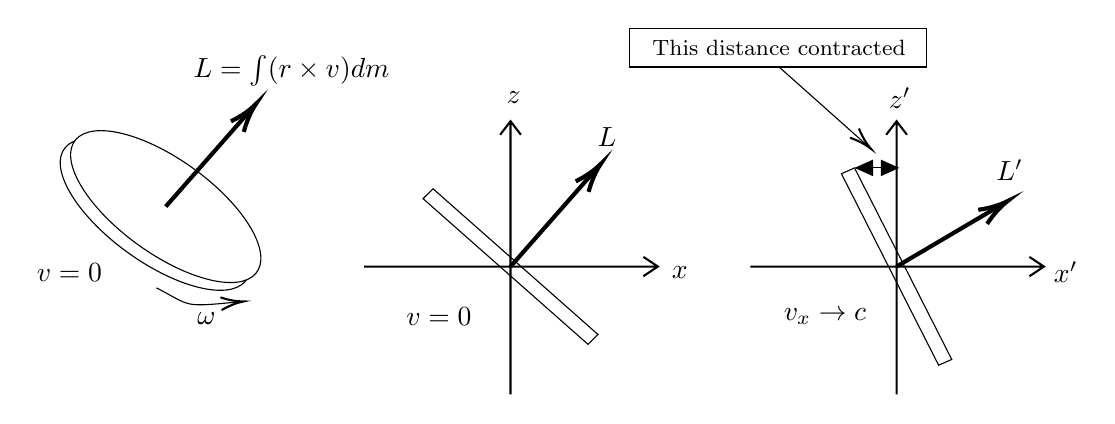
\begin{tikzpicture}[x=0.75pt,y=0.7pt,yscale=-1,xscale=1]
%uncomment if require: \path (0,300); %set diagram left start at 0, and has height of 300

%Shape: Ellipse [id:dp6696584947764774] 
\draw   (105.99,95.55) .. controls (114.14,85.31) and (140.18,92.46) .. (164.14,111.53) .. controls (188.1,130.6) and (200.92,154.36) .. (192.77,164.6) .. controls (184.62,174.85) and (158.58,167.7) .. (134.62,148.63) .. controls (110.66,129.56) and (97.84,105.8) .. (105.99,95.55) -- cycle ;
%Shape: Ellipse [id:dp8843951455763316] 
\draw  [fill={rgb, 255:red, 255; green, 255; blue, 255 }  ,fill opacity=1 ] (110.99,91.55) .. controls (119.14,81.31) and (145.18,88.46) .. (169.14,107.53) .. controls (193.1,126.6) and (205.92,150.36) .. (197.77,160.6) .. controls (189.62,170.85) and (163.58,163.7) .. (139.62,144.63) .. controls (115.66,125.56) and (102.84,101.8) .. (110.99,91.55) -- cycle ;
%Straight Lines [id:da6714691596952527] 
\draw [line width=1.5]    (154.38,126.08) -- (196,75.35) ;
\draw [shift={(197.9,73.03)}, rotate = 489.37] [color={rgb, 255:red, 0; green, 0; blue, 0 }  ][line width=1.5]    (14.21,-4.28) .. controls (9.04,-1.82) and (4.3,-0.39) .. (0,0) .. controls (4.3,0.39) and (9.04,1.82) .. (14.21,4.28)   ;

%Curve Lines [id:da608409716212424] 
\draw    (149.9,168.03) .. controls (167.54,177.83) and (162.13,178.03) .. (190.14,175.21) ;
\draw [shift={(191.9,175.03)}, rotate = 534.29] [color={rgb, 255:red, 0; green, 0; blue, 0 }  ][line width=0.75]    (10.93,-3.29) .. controls (6.95,-1.4) and (3.31,-0.3) .. (0,0) .. controls (3.31,0.3) and (6.95,1.4) .. (10.93,3.29)   ;

%Shape: Rectangle [id:dp2988248655701031] 
\draw  [fill={rgb, 255:red, 255; green, 255; blue, 255 }  ,fill opacity=1 ] (283.18,116.89) -- (362.64,192.09) -- (357.82,197.17) -- (278.36,121.98) -- cycle ;
%Shape: Axis 2D [id:dp3998228460871881] 
\draw [line width=0.75]  (250,157.03) -- (391.5,157.03)(320.5,82) -- (320.5,223.03) (384.5,152.03) -- (391.5,157.03) -- (384.5,162.03) (315.5,89) -- (320.5,82) -- (325.5,89)  ;
%Straight Lines [id:da08204495575914073] 
\draw [line width=1.5]    (320.5,157.03) -- (362.12,106.31) ;
\draw [shift={(364.02,103.99)}, rotate = 489.37] [color={rgb, 255:red, 0; green, 0; blue, 0 }  ][line width=1.5]    (14.21,-4.28) .. controls (9.04,-1.82) and (4.3,-0.39) .. (0,0) .. controls (4.3,0.39) and (9.04,1.82) .. (14.21,4.28)   ;

%Shape: Rectangle [id:dp9756203932975158] 
\draw  [fill={rgb, 255:red, 255; green, 255; blue, 255 }  ,fill opacity=1 ] (486.24,106.1) -- (533.08,204.97) -- (526.76,207.96) -- (479.92,109.1) -- cycle ;
%Shape: Axis 2D [id:dp2253494066411521] 
\draw [line width=0.75]  (436,157.03) -- (577.5,157.03)(506.5,82) -- (506.5,223.03) (570.5,152.03) -- (577.5,157.03) -- (570.5,162.03) (501.5,89) -- (506.5,82) -- (511.5,89)  ;
%Straight Lines [id:da26681235965231986] 
\draw [line width=1.5]    (506.5,157.03) -- (557.46,124.84) ;
\draw [shift={(560,123.23)}, rotate = 507.72] [color={rgb, 255:red, 0; green, 0; blue, 0 }  ][line width=1.5]    (14.21,-4.28) .. controls (9.04,-1.82) and (4.3,-0.39) .. (0,0) .. controls (4.3,0.39) and (9.04,1.82) .. (14.21,4.28)   ;

%Straight Lines [id:da2736459794596652] 
\draw    (489.24,106.1) -- (504.8,106.1) ;
\draw [shift={(507.8,106.1)}, rotate = 180] [fill={rgb, 255:red, 0; green, 0; blue, 0 }  ][line width=0.08]  [draw opacity=0] (8.93,-4.29) -- (0,0) -- (8.93,4.29) -- cycle    ;
\draw [shift={(486.24,106.1)}, rotate = 0] [fill={rgb, 255:red, 0; green, 0; blue, 0 }  ][line width=0.08]  [draw opacity=0] (8.93,-4.29) -- (0,0) -- (8.93,4.29) -- cycle    ;
%Straight Lines [id:da8576239603286319] 
\draw    (450.13,54.23) -- (492.69,94.85) ;
\draw [shift={(494.13,96.23)}, rotate = 223.67000000000002] [color={rgb, 255:red, 0; green, 0; blue, 0 }  ][line width=0.75]    (10.93,-3.29) .. controls (6.95,-1.4) and (3.31,-0.3) .. (0,0) .. controls (3.31,0.3) and (6.95,1.4) .. (10.93,3.29)   ;


% Text Node
\draw (174,184) node    {$\omega $};
% Text Node
\draw (108,160) node    {$v=0$};
% Text Node
\draw (402,160) node    {$x$};
% Text Node
\draw (322,70) node    {$z$};
% Text Node
\draw (215,56) node    {$L=\int ( r\times v) dm$};
% Text Node
\draw (367,90) node    {$L$};
% Text Node
\draw (286,183) node    {$v=0$};
% Text Node
\draw (588,160) node    {$x'$};
% Text Node
\draw (508,70) node    {$z'$};
% Text Node
\draw (561,107) node    {$L^{\prime }$};
% Text Node
\draw (472,183) node    {$v_{x}\rightarrow c$};
% Text Node
\draw    (378,34) -- (521,34) -- (521,54) -- (378,54) -- cycle  ;
\draw (449.87,44) node  [font=\footnotesize] [align=left] {This distance contracted};


\end{tikzpicture}
    \caption{Spinning disk}
    \label{fig:spinning-disk}
\end{figure}
The closer the disk gets to the speed of light, the more the disk surface appears in the observer's frame to align normal to the velocity direction. In the rest frame translating with the disk itself, the disk still appears aligned in the original way. In the observer's frame, though, the angular momentum L appears to turn toward the direction of the velocity becoming $L^{\prime}$. The greater the speed, the greater this turning. At light speed, $L^{\prime}$ and $v$ become parallel.

Quantum mechanically, then, \bluep{at high speed, a particle's angular momentum (spin) magnitude remains unchanged, but its direction appears to us in our frame to realign itself closer to that of the translational velocity vector.}

Mathematically, these kinds of relativistic complications are incorporated into the form of the spinors $u_{r}(\mathrm{p})$ and $v_{r}(\mathrm{p})$ (by their dependence on 3 -momentum and thus ultimately, on velocity) and by how they are combined to form more general spin states.

\begin{qt}
\redp{Note that the spinor components are actually dependent on particle velocity, rather than momentum, by the following logic.} Energy and momentum are expressed (in non-natural units to make it easier to understand)
$$
E=\frac{m c^{2}}{\sqrt{1-v^{2} / c^{2}}} \quad p^{i}=\frac{m v^{i}}{\sqrt{1-v^{2} / c^{2}}}
$$
so in the coefficient and spinor components of the Dirac spinor (\ref{four-spinors}) the mass $m$ drops out. This leaves them a function solely of velocity.
\end{qt}

\subsubsection{What happens when the particle is not stationary}
Note what happens to the spin as seen by us, for an electron whose spin is represented solely by
$u_{1},$ but has $p^{1} \neq 0,$ with $p^{2}=p^{3}=0$ in our frame (the lab.)
$$
\Sigma_{3}\left|\psi^{(1)}\right\rangle=\frac{1}{2}\left[\begin{array}{cccc}
{1} & {} \\
{} & {-1} \\
{} & {} & {1} \\
{} & {} & {}&{-1}
\end{array}\right] \frac{E+m}{2 m}\left(\begin{array}{c}
{1} \\
{0} \\
{0} \\
{\frac{p^{1}}{E+m}}
\end{array}\right) e^{-f p x}=\frac{1}{2} \sqrt{\frac{E+m}{2 m}}\left(\begin{array}{c}
{1} \\
{0} \\
{0} \\
{\frac{-p^{1}}{E+m}}
\end{array}\right) e^{-i p x} \neq \frac{1}{2}\left|\psi^{(1)}\right\rangle
$$
\textbf{\redp{$u_1$ for a non-translating electron has spin up, but $u_1$ for an electron with high trnasverse velocity is not an up eigenstate.}}

Now consider $u_1$ representing an electron traveling in the $z$ direction instead of the x direction
$$
\Sigma_{3}\left|\psi^{(1)}\right\rangle=\frac{1}{2}\left[\begin{array}{cccc}
{1} \\
{} & {-1} \\
{} & {} & {1} \\
{} & {} & {} & {-1}
\end{array}\right]\sqrt{\frac{E+m}{2 m}}\left(\begin{array}{c}
{1} \\
{0} \\
{p^{3}} \\
{\frac{p^{3}}{E+m}} \\
{0}
\end{array}\right) e^{-t p x}=\frac{1}{2} \sqrt{\frac{E+m}{2 m}}\left(\begin{array}{c}
{1} \\
{0} \\
{\frac{p^{3}}{E+m}} \\
{0}
\end{array}\right) e^{-i p x}=\frac{1}{2}\left|\psi^{(1)}\right\rangle
$$
This electron, represented by $u_{1},$ is an up eigenstate as it moves, just as it was when it was at rest. Relativistically, this makes sense, as the plane of a spinning disk with $\mathbf{L}$ aligned in the direction of $\mathbf{p}$ would not appear to turn as $\mathbf{p}$ increased from zero to a relativistic value.

\redp{\textbf{In general, boosts in the spin axis direction leave $u_{1}, u_{2}, v_{2}$ and $v_{1}$ in the same spin eigenstates as they would be at rest. Boosts in other directions take them out of these spin eigenstates.}}

\begin{mybox}
\textbf{The four-spinors span the 4D spinor space}

By analogy, we can surmise that the four Dirac spinors $u_{1}, u_{2}, v_{2}$ and $v_{1}$ of (\ref{four-spinors}) span the $\mathrm{RQM}$ 4D spinor space of all possible spins and momenta, and thus, are basis vectors for that space. Our RQM general solution (\ref{general-Dirac-state}) contains within it all possible relativistic spin states.

More mathematically, we should know that a $4 \mathrm{D}$ space is spanned by four column vectors, where these vectors are all independent of one another. Generally. the vector solutions of an eigenvalue problem, which is what the Dirac equation solutions are, are independent and complete, and thus we can conclude, span the space. They can be used as basis vectors.
\end{mybox}
\subsubsection{General RQM solution contains all possible spin directions}
In (\ref{general-Dirac-state}), different coefficients $C_{1}(\mathbf{p})$ and $\mathcal{C}_{2}(\mathbf{p})$ will yield different spin states for C type particles. And different coefficients $D^{\dagger}_{1(\mathbf{p})}$ and $D^{\dagger}_{2(\mathbf{p})}$ will yield different spin states for $D$ type particles.

To see how this works, we consider how each of the four states shown below can be represented by their respective terms in the general particle state solution (\ref{general-Dirac-state}). 
\begin{figure}[H]
    \centering
\tikzset{every picture/.style={line width=0.75pt}} %set default line width to 0.75pt        

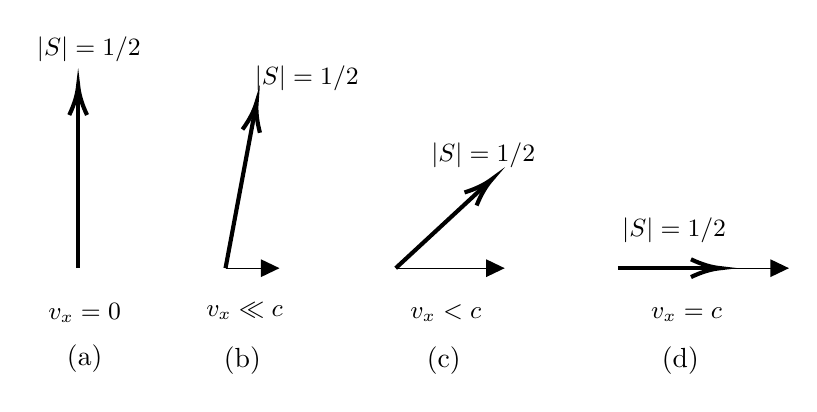
\begin{tikzpicture}[x=0.75pt,y=0.75pt,yscale=-1,xscale=1]
%uncomment if require: \path (0,300); %set diagram left start at 0, and has height of 300

%Straight Lines [id:da533603137195499] 
\draw [line width=1.5]    (79.87,190.5) -- (79.87,105.5) ;
\draw [shift={(79.87,102.5)}, rotate = 450] [color={rgb, 255:red, 0; green, 0; blue, 0 }  ][line width=1.5]    (14.21,-4.28) .. controls (9.04,-1.82) and (4.3,-0.39) .. (0,0) .. controls (4.3,0.39) and (9.04,1.82) .. (14.21,4.28)   ;

%Straight Lines [id:da31466198885223695] 
\draw    (150.87,190.5) -- (173.87,190.5) ;
\draw [shift={(176.87,190.5)}, rotate = 180] [fill={rgb, 255:red, 0; green, 0; blue, 0 }  ][line width=0.08]  [draw opacity=0] (8.93,-4.29) -- (0,0) -- (8.93,4.29) -- cycle    ;

%Straight Lines [id:da6431925700861189] 
\draw [line width=1.5]    (150.87,190.5) -- (165.31,113.45) ;
\draw [shift={(165.87,110.5)}, rotate = 460.62] [color={rgb, 255:red, 0; green, 0; blue, 0 }  ][line width=1.5]    (14.21,-4.28) .. controls (9.04,-1.82) and (4.3,-0.39) .. (0,0) .. controls (4.3,0.39) and (9.04,1.82) .. (14.21,4.28)   ;

%Straight Lines [id:da8282450907912188] 
\draw    (232.87,190.5) -- (282.37,190.5) ;
\draw [shift={(285.37,190.5)}, rotate = 180] [fill={rgb, 255:red, 0; green, 0; blue, 0 }  ][line width=0.08]  [draw opacity=0] (8.93,-4.29) -- (0,0) -- (8.93,4.29) -- cycle    ;

%Straight Lines [id:da09697600465348566] 
\draw [line width=1.5]    (232.87,190.5) -- (277.16,149.54) ;
\draw [shift={(279.37,147.5)}, rotate = 497.24] [color={rgb, 255:red, 0; green, 0; blue, 0 }  ][line width=1.5]    (14.21,-4.28) .. controls (9.04,-1.82) and (4.3,-0.39) .. (0,0) .. controls (4.3,0.39) and (9.04,1.82) .. (14.21,4.28)   ;

%Straight Lines [id:da13695386046952507] 
\draw    (339.87,190.5) -- (419.33,190.5) ;
\draw [shift={(422.33,190.5)}, rotate = 180] [fill={rgb, 255:red, 0; green, 0; blue, 0 }  ][line width=0.08]  [draw opacity=0] (8.93,-4.29) -- (0,0) -- (8.93,4.29) -- cycle    ;

%Straight Lines [id:da04790853968035602] 
\draw [line width=1.5]    (339.87,190.5) -- (386.33,190.5) ;
\draw [shift={(389.33,190.5)}, rotate = 180] [color={rgb, 255:red, 0; green, 0; blue, 0 }  ][line width=1.5]    (14.21,-4.28) .. controls (9.04,-1.82) and (4.3,-0.39) .. (0,0) .. controls (4.3,0.39) and (9.04,1.82) .. (14.21,4.28)   ;


% Text Node
\draw (85,85.07) node  [font=\small]  {$|S|=1/2$};
% Text Node
\draw (83,212.07) node  [font=\small]  {$v_{x} =0$};
% Text Node
\draw (160,211.07) node  [font=\small]  {$v_{x} \ll c$};
% Text Node
\draw (257,212.07) node  [font=\small]  {$v_{x} < c$};
% Text Node
\draw (373,213.07) node  [font=\small]  {$v_{x} =c$};
% Text Node
\draw (190,99.07) node  [font=\small]  {$|S|=1/2$};
% Text Node
\draw (275,136.07) node  [font=\small]  {$|S|=1/2$};
% Text Node
\draw (367,172.07) node  [font=\small]  {$|S|=1/2$};
% Text Node
\draw (83,234.07) node   [align=left] {(a)};
% Text Node
\draw (159,235.07) node   [align=left] {(b)};
% Text Node
\draw (256,235.07) node   [align=left] {(c)};
% Text Node
\draw (370,235.07) node   [align=left] {(d)};


\end{tikzpicture}

    \caption{Effect of Transverse Velocity on Dirac Particle Spin}
    \label{fig:transverse-velocity-effect}
\end{figure}

In general, for $j=a,b,c,d$, the four states shown (for a C type particle) in the figure are
\begin{equation}
\left|\psi_{(j)}\right\rangle=\sqrt{\frac{m}{V E_{p_{j}}}}\left(C_{1}\left(p_{j}\right) u_{1}\left(p_{j}\right)+C_{2}\left(p_{j}\right) u_{2}\left(p_{j}\right)\right) e^{-i p_{j} x}
\label{psi-abcd}
\end{equation}
Not that we have a particle here (so no $D$ type terms), and $\mathbf{p}_j$ is known. State (a) there is effectively spin up with $\mathrm{p}_{\mathrm{a}}=0$, so
\begin{equation}
\left|\psi_{(a)}\right\rangle=\sqrt{\frac{m}{V E_{p_{a}}}} C_{1}(0) u_{1}(0) e^{-i p_{a} x}=\sqrt{\frac{m}{V E_{\mathrm{p}_{a}}}} \sqrt{\frac{E_{\mathrm{p}_{a}}+m}{2 m}}\left(\begin{array}{l}
{\mathrm{I}} \\
{0} \\
{0} \\
{0}
\end{array}\right) e^{-i p_{a} x}
\end{equation}
which is an eigenstate of $\Sigma_3$. So for state (a), $|\psi_a\rangle$ has $C_1=1$ and $C_2=0$.

For the last state (d), where the particle is traveling at the speed of light, (\ref{psi-abcd}) becomes an eigenstate of $\Sigma_1$ with eigenvalue $1/2$,
$$
\left|\psi_{(d)}\right\rangle=\sqrt{\frac{m}{V E_{\mathrm{p}_{d}}}} C_{1}(\infty) u_{1}(\infty) e^{-i p_{d} x}+\sqrt{\frac{m}{V E_{\mathrm{p} d}}} C_{2}(\infty) u_{2}(\infty) e^{-i p_{d} x}
$$
$$
=\sqrt{\frac{m}{V E_{\mathrm{p}_{d}}}} \sqrt{\frac{E_{\mathrm{p}_{d}}+m}{2 m}}\left(\begin{array}{l}
{1} \\
{1} \\
{1} \\
{1}
\end{array}\right) e^{-i p_{d} x}
$$
where here, we must have $C_1=C_2=1$. (in the normalized version, $C_1=C_2=1/\sqrt{2}$).For "in between" states $(b)$ and $(c), C_{1}$ and $C_{2}$ would have other values. The bottumline is:\redp{$\mathbf{p}$ determines $u_{1,2}$ and then spin is represented by correct linear combination of $u_1$ and $u_2$}. Note that \bluep{we can never have a relativistic state where the spin vector and $\mathbf{p}$ are at right angles.}

Note that $u_{1}$ and $u_{2}$ actually exist in spinor space (they are spinor space basis vectors in that space), but they correspond to directions in physical space. For example, in the at-rest system, $u_1$ represents spin up and so can be visualized as a spatial vector that points in the $+z$ direction. Similarly, in the at-rest system, $u_{2}$ represents spin down, so can be visualized as a vector pointing in the $-z$ direction. 
\begin{qt}
\underline{Summary}

1. $u_{1}(\mathrm{p}) e^{-i p x}$ and  $u_{2}(\mathrm{p}) e^{-i p x}$ is each always an eigenstate of the Dirac equation (for any $\mathbf{p}$)

2. $u_{1}(\mathrm{p}) e^{-i p x}$ and $u_{2}(\mathrm{p}) e^{-i p x}$ is each sometimes an eigenstate of $z$ spin, i.e. of $\Sigma_{3}\left(\text { for } \mathbf{p}=0 \text { or }=p^{3} \mathbf{i}_{3}\right)$

3. $u_{1}(\mathbf{p}) e^{-i p x}$ and $u_{2}(\mathbf{p}) e^{-i p x}$ are always basis vectors for any general state $|\psi\rangle$ (for any $\mathbf{p}$ )

4. $u_{1}(p)$ and $u_{2}(p)$ is each sometimes an eigenstate of $z$ spin, i.e. of $\Sigma_{3}$ for $\mathbf{p}=0$ or$=p^{3} \mathbf{i}_{3}$)

5. $u_{1}(\mathbf{p})$ and $u_{2}(\mathbf{p})$ are always basis vectors in $4 \mathrm{D}$ spinor space (for any $\mathbf{p}$) 

6. \textbf{$u_{1}(\mathrm{p})$ and $u_{2}(\mathrm{p})$ change orientation, as visualized in physical space, as $\mathrm{p}$ changes.}

7. Spin S (often in relativity as $\Sigma$ ) changes direction with p, but differently than $u_{1}$ and $u_{2}$
\end{qt}
Any general spin state $u$ can be represented as a linear combination of $u_{1}$ and  $u_{2}$ (for any $\mathbf{p}$)
$$
u(\mathrm{p})=C_{1}(\mathrm{p}) u_{1}(\mathrm{p})+C_{2}(\mathrm{p}) u_{2}(\mathrm{p})
$$
Any general particle state includes a spin part plus a spacetime part(for any given $\mathbf{p}$):
$$
\left|\psi_{\mathfrak{p}}\right\rangle=\sqrt{\frac{m}{2 V E_{\mathrm{p}}}} u(\mathbf{p}) e^{-i p x}=\sqrt{\frac{m}{2 V E_{\mathrm{p}}}}\left(C_{1}(\mathrm{p}) u_{1}(\mathrm{p}) e^{-i p x}+C_{2}(\mathrm{p}) u_{2}(\mathrm{p}) e^{-i p x}\right)
$$
\subsection{RQM Helicity operator}
For massless particles ($v=c$), the velocity vector must perfectly align with the spin vector. This alignment is called \textbf{perfect helicity}. In general, if the spin axis (using the right-hand rule), of a particle is in the direction of $v$ one
says the particle has \textbf{positive helicity}. If spin points in the direction of $- v$, the particle has \textbf{negative helicitv}. 

The degree  of helicity a particle has be define in terms of the angle between the spin vector and the velocity vector. It is maximum if that angle is zero.\textbf{ The dot product of the spin vector with a unit vector in the $\mathbf{p}$ (or equivalently, the $v$) direction has come to be the mathematical definition of helicity}.

\bluep{Our spin operator $\Sigma$ in RQM plays the role of a 3-vector in physical space that points in the direction of spin.} The inner product in physical space of the spin operator $\Sigma$ and the unit vector in the $\mathbf{p}$ direction would then be \textbf{helicity operator}:
\begin{qt}
\begin{equation}
\Sigma_{p}=\Sigma \cdot i_{p}=\Sigma \cdot \frac{p}{|p|}=\Sigma_{1} \frac{p^{1}}{|p|}+\Sigma_{2} \frac{p^{2}}{|p|}+\Sigma_{3} \frac{p^{3}}{|p|}
\label{helicity-operator}
\end{equation}
(\ref{helicity-operator}) is a $4\times4$ matrix in spinor space because each $\Sigma_i$ is a matrix. (\ref{helicity-operator}) is a scalar in physical space because it is the inner product of two vectors.
\end{qt}
\begin{example}
Consider a case where a particle is in the first eigenstate of (\ref{four-spinors}), and if $p^3\neq0$, we have
$$
\Sigma \cdot \frac{\mathbf{p}}{|\mathbf{p}|}\left|\psi^{(1)}\right\rangle=\Sigma_{3} \underbrace{\frac{p^{3}}{|\mathbf{p}|}}_{=1}\left|\psi^{(1)}\right\rangle=\frac{1}{2}\left[\begin{array}{cccc}
{1} \\
{} & {-1} \\
{} & {} & {1} \\
{} & {} & {} & {-1}
\end{array}\right]\sqrt{\frac{E+m}{2 m}}\left(\begin{array}{c}
{1} \\
{0} \\
{\frac{p^3}{E+m}} \\
{0}
\end{array}\right)e^{-ipx}=\frac{1}{2}\left|\psi^{(1)}\right\rangle
$$
\end{example}
\begin{example}
Note that if $p^3$ were negative (-z direction)
$$
\Sigma_{3}\left|\psi^{(1)}\right\rangle=\frac{1}{2}\left[\begin{array}{cccc}
{1} \\
{} & {-1} \\
{} & {} & {1} \\
{} & {} & {} & {-1}
\end{array}\right]\sqrt{\frac{E+m}{2 m}}\left(\begin{array}{c}
{1} \\
{0} \\
{\frac{p^{3}}{E+m}} \\
{0}
\end{array}\right) e^{-i p x}=\frac{1}{2}\left|\psi^{(1)}\right\rangle
$$
but
$$
\Sigma \cdot \frac{\mathbf{p}}{|\mathbf{p}|}\left|\psi^{(1)}\right\rangle=\Sigma_{3} \underbrace{\frac{p^{3}}{|\mathbf{p}|}}_{=-1}\left|\psi^{(1)}\right\rangle=-\frac{1}{2}\left|\psi^{(1)}\right\rangle
$$
\end{example}
In general, a $+1 / 2$ helicity state for spinors means the spin is in the direction of $p$; a $-1 / 2$ helicity eigenvalue means spin is in the direction of $-p$.

\section{The Dirac Equation in QFT}
The Dirac equation for fields (where we will, as with scalar fields, work in the Heisenberg picture), is
\begin{equation}
\left(i \gamma^{\mu} \partial_{\mu}-m\right) \psi=0
\end{equation}
Its eigensolutions
\begin{equation}
\psi^{(1)}=u_{1} e^{-i p x} \quad \psi^{(2)}=u_{2} e^{-i p x} \quad \psi^{(3)}=v_{2} e^{i p x} \quad \psi^{(4)}=v_{1} e^{i p x}
\end{equation}
\textbf{\underline{The adjoint Dirac equation for fields is}}
\begin{equation}
i \partial_{\mu} \bar{\psi} \gamma^{\mu}+m \bar{\psi}=0
\end{equation}
with adjoint eigensolutions
\begin{equation}
\bar{\psi}=\psi^{\dagger} \gamma^{0} \rightarrow \bar{\psi}^{(1)}=u_{1}^{\dagger} \gamma_{e}^{0} e^{i p x}=\bar{u}_{\mathrm{l}} e^{i p x} \quad \bar{\psi}^{(2)}=\bar{u}_{2} e^{i \phi x} \quad \bar{\psi}^{(3)}=\bar{v}_{2} e^{-i \varphi x} \quad \bar{\psi}^{(4)}=\bar{v}_{1} e^{-\dot{\varphi} x}
\end{equation}
\begin{qt}
the general discrete plane wave solutions are
\begin{equation}
\begin{aligned}
\psi &=\sum_{r, \mathbf{p}} \sqrt{\frac{m}{V E_{\mathrm{p}}}}\left(c_{r}(\mathbf{p}) u_{r}(\mathbf{p}) e^{-i p x}+d_{r}^{\dagger}(\mathbf{p}) v_{r}(\mathbf{p}) e^{i p x}\right) \\
&=\quad \psi^{+} \quad+\quad \psi^{-}
\end{aligned}
\end{equation}
\begin{equation}
\begin{aligned}
&\bar{\psi}=\sum_{r, p} \sqrt{\frac{m}{V E_{p}}}\left(d_{r}(p) \bar{v}_{r}(p) e^{-i p x}+c_{r}^{\dagger}(p) \bar{u}_{r}(p) e^{i p x}\right)\\
&=\quad \bar{\psi}^{+} \quad+\quad \bar{\psi}^{-}
\end{aligned}
\end{equation}
\end{qt}
The general continuous plane wave solutions are
\begin{equation}
\begin{aligned}
&\psi=\sum_{r} \sqrt{\frac{m}{(2 \pi)^{3}}} \int \frac{d^{3} \mathbf{p}}{\sqrt{E_{p}}}\left(c_{r}(\mathbf{p}) u_{r}(\mathbf{p}) e^{-i p x}+d_{r}^{\dagger}(\mathbf{p}) v_{r}(\mathbf{p}) e^{i p x}\right)\\
&\bar{\psi}=\sum_{r} \sqrt{\frac{m}{(2 \pi)^{3}}} \int \frac{d^{3} \mathbf{p}}{\sqrt{E_{p}}}\left(d_{r}(\mathbf{p}) \bar{v}_{r}(\mathbf{p}) e^{-i p x}+c_{r}^{\dagger}(\mathbf{p}) \bar{u}_{r}(\mathbf{p}) e^{i p x}\right)
\end{aligned}
\end{equation}
\begin{qt}
the Lagrangian ( density) for free spinor fields to be
\begin{equation}
\mathcal{L}_{0}^{1/2}=\bar{\psi}\left(i \gamma^{\alpha} \partial_{\alpha}-m\right) \psi
\end{equation}
Conjugate momenta for $\psi$ and $\bar{\psi}$ are
\begin{equation}
\pi^{1 / 2}=\frac{\partial \mathcal{L}_{0}^{1 / 2}}{\partial \psi_{0}}=i \psi \gamma^{0}=i \psi^{\dagger} \gamma^{\dagger} \gamma^{0}=i \psi^{\dagger}
\end{equation}
\begin{equation}
\bar{\pi}^{1 / 2}=\frac{\partial \mathcal{L}_{0}^{1 / 2}}{\partial \bar{\psi}_{, 0}}=0
\end{equation}
The Dirac Hamiltonian density can be found from the Legendre transformation as
\begin{equation}
\begin{aligned}
\mathcal{H}_{0}^{1 / 2} &=\pi^{1 / 2} \dot{\psi}+\bar{\pi}^{1 / 2} \dot{\bar{\psi}}-\mathcal{L}_{0}^{1 / 2}=i \psi^{\dagger} \dot{\psi}-\mathcal{L}_{0}^{1 / 2}=i \underbrace{\psi^{\dagger} \gamma^{0}}_{\bar{\psi}} \gamma^{0} \dot{\psi}-\mathcal{L}_{0}^{1 / 2} \\
&=i \bar{\psi} \gamma^{0} \dot{\psi}\underbrace{-i \bar{\psi} \gamma^{0} \dot{\psi}-i \bar{\psi} \gamma^{i} \partial_{i} \psi}_{-i\bar{\psi}\gamma^{\alpha}\partial_{\alpha}\psi}+m \bar{\psi} \psi=-i \bar{\psi} \gamma^{i} \partial_{i} \psi+m \bar{\psi} \psi
\end{aligned}
\end{equation}
\end{qt}
\section{Anti-commutation Relations for Dirac Fields}
\begin{qt}
\begin{equation}
    \left[c_{r}(\mathbf{p}), c_{s}^{\dagger}\left(\mathbf{p}^{\prime}\right)\right]_{+}=\left[d_{r}(\mathbf{p}), d_{s}^{\dagger}\left(\mathbf{p}^{\prime}\right)\right]_{+}=\delta_{r S} \delta_{\mathbf{p p}^{\prime}}(\text { discrete }) ;=\delta_{r s} \delta(\mathbf{p - p ^ { \prime }})(\text { continuous })
\end{equation}
All other anti-commutators between coefficients equal zero.
\end{qt}
\section{The Dirac Hamiltonian in QFT}
Similar to what we did for scalar fields, we find the Dirac Hamiltonian by integrating the Dirac Hamiltonian density over all space (a volume V containing the discrete solutions, which we can make as large as we like), i.e.,
\begin{equation}
H_{0}^{1 / 2}=\int \mathcal{H}_{0}^{1 / 2} d^{3} x=\int\left(-i \bar{\psi} \gamma^{i} \partial_{i} \psi+m \bar{\psi} \psi\right) d^{3} x
\label{Dirac-Hamiltonian}
\end{equation}
we substitute the Dirac general solution into (\ref{Dirac-Hamiltonian}) to give
$$
\begin{aligned}
&H_{0}^{1 / 2}=\int\left(-i \bar{\psi} \gamma^{i} \partial_{i} \psi+m \bar{\psi} \psi\right) d^{3} x=\\
&\int\left(\sum_{r, p} \sqrt{\frac{m}{V E_{p}}}\left(d_{r}(p) \bar{v}_{r}(\mathbf{p}) e^{-i p x}+c_{r}^{\dagger}(\mathbf{p}) \bar{u}_{r}(\mathbf{p}) e^{i p x}\right)\right) \times
\end{aligned}
$$
$$
\left(-i \gamma^{i} \partial_{i}\right)\left(\sum_{s, p^{\prime}} \sqrt{\frac{m}{V E_{p^{\prime}}}}\left(c_{s}\left(\mathbf{p}^{\prime}\right) u_{s}\left(\mathbf{p}^{\prime}\right) e^{-i p^{\prime} x}+d_{s}^{\dagger}\left(\mathbf{p}^{\prime}\right) v_{s}\left(\mathbf{p}^{\prime}\right) e^{i p^{\prime} x}\right)\right) d^{3} x
$$
$$
+\int m\left(\sum_{r, p} \sqrt{\frac{m}{V E_{p}}}\left(d_{r}(p) \bar{v}_{r}(p) e^{-i p x}+c_{r}^{\dagger}(p) \bar{u}_{r}(p) e^{i p x}\right)\right) \times
$$
$$
\left(\sum_{s, \mathbf{p}^{\prime}} \sqrt{\frac{m}{V E_{\mathbf{p}^{\prime}}}}\left(c_{s}\left(\mathbf{p}^{\prime}\right) u_{s}\left(\mathbf{p}^{\prime}\right) e^{-i p^{\prime} x}+d_{s}^{\dagger}\left(\mathbf{p}^{\prime}\right) v_{s}\left(\mathbf{p}^{\prime}\right) e^{i \mathbf{p}^{\prime} \cdot x}\right)\right) d^{3} x
$$
The first of the two integrals above becomes
$$
 \int\left(\sum_{r, \mathbf{p}} \sqrt{\frac{m}{V E_{p}}}d_{r}(\mathbf{p}) \bar{v}_{r}(\mathbf{p}) e^{-i\left(E_{p} t-p^{i} x^{i}\right)}\right)\left(\sum_{s, p^{\prime}} \sqrt{\frac{m}{V E_{p^{\prime}}}} c_{s}\left(\mathbf{p}^{\prime}\right) \gamma^{i} \underbrace{p^{\prime i}}_{\text { from }\partial_i} u_{s}\left(\mathbf{p}^{\prime}\right) e^{-i\left(E_{p^{\prime}}-p^{\prime i} x^{i}\right)}\right)d^3x
$$
$$
+\int\left(\sum_{r, \mathrm{p}} \sqrt{\frac{m}{V E_{\mathrm{p}}}} d_{r}(\mathrm{p}) \bar{v}_{r}(\mathbf{p}) e^{-i\left(E_{\mathrm{p}} t-p^{i} x^{i}\right)}\right)\left(\sum_{s, p^{\prime}} \sqrt{\frac{m}{V E_{p^{\prime}}}} d_{s}^{\dagger}\left(p^{\prime}\right) \gamma^{i}\left(-p^{\prime i}\right) v_{s}\left(p^{\prime}\right) e^{i\left(E_{p^{\prime}}t-p^{\prime i} x^{i}\right)}\right) d^{3} x
$$
$$
+\int\left(\sum_{r, \mathrm{p}} \sqrt{\frac{m}{V E_{\mathrm{p}}}} c^{\dagger}_{r}(\mathrm{p}) \bar{u}_{r}(\mathbf{p}) e^{-i\left(E_{\mathrm{p}} t-p^{i} x^{i}\right)}\right)\left(\sum_{s, p^{\prime}} \sqrt{\frac{m}{V E_{p^{\prime}}}} c_{s}\left(p^{\prime}\right) \gamma^{i}\left(p^{\prime i}\right) u_{s}\left(p^{\prime}\right) e^{i\left(E_{p^{\prime}}t-p^{\prime i} x^{i}\right)}\right) d^{3} x
$$
$$
+\int\left(\sum_{r, \mathrm{p}} \sqrt{\frac{m}{V E_{\mathrm{p}}}} c^{\dagger}_{r}(\mathrm{p}) \bar{u}_{r}(\mathbf{p}) e^{-i\left(E_{\mathrm{p}} t-p^{i} x^{i}\right)}\right)\left(\sum_{s, p^{\prime}} \sqrt{\frac{m}{V E_{p^{\prime}}}} d^{\dagger}_{s}\left(p^{\prime}\right) \gamma^{i}\left(-p^{\prime i}\right) v_{s}\left(p^{\prime}\right) e^{i\left(E_{p^{\prime}}t-p^{\prime i} x^{i}\right)}\right) d^{3} x
$$
\redp{because an integral over all space of the oscillating function $e^{if(\mathbf{x})}$, where $f(\mathbf{x}\neq0)$ is zero. }So,in the first and last lines, only terms with $\mathbf{p}=-\mathbf{p}^{\prime}$ will survive. And in the $2^{\text {nd }}$ and $3^{\text {rd }}$ lines, only terms in $\mathbf{p}^{\prime}=\mathbf{p}$ will. We assume, as in $\mathrm{RQM},$ that \textbf{\redp{the order of spinors and coefficients (such as $c_{r} \text { and } d_{r}$) can be interchanged at will, but we must preserve the order of spinor entities as it represent matrix/vector multiplication in spinor space.}}
$$
+\int\left[\sum_{r, s, \mathbf{p}} \frac{m}{V E_{\mathbf{p}}} d_{r}(-\mathbf{p}) \bar{v}_{r}(-\mathbf{p}) \gamma^{i} p^{i} u_{s}(\mathbf{p}) c_{s}(\mathbf{p}) e^{-i 2 E_{p} t}\right] d^{j}
$$
$$
+\int\left(\sum_{r, s, \mathbf{p}} \frac{m}{V E_{\mathrm{p}}} d_{r}(\mathbf{p}) \bar{v}_{r}(\mathbf{p}) \gamma^{i}\left(-p^{i}\right) v_{s}(\mathbf{p}) d_{s}^{\dagger}(\mathbf{p})\right) d^{3} x
$$
$$
+\int\left(\sum_{r, s, \mathbf{p}} \frac{m}{V E_{p}} c_{r}^{\dagger}(\mathbf{p}) \bar{u}_{r}(\mathbf{p}) \gamma^{i} p^{i} u_{s}(\mathbf{p}) c_{s}(\mathbf{p})\right) d^{3} x
$$
$$
+\int\left(\sum_{r, s, \mathbf{p}} \frac{m}{V E_{p}} c_{r}^{\dagger}(-\mathbf{p}) \bar{u}_{r}(-\mathbf{p}) \gamma^{i}\left(-p^{i}\right) v_{s}(\mathbf{p}) d_{s}^{\dagger}(\mathbf{p}) e^{i 2 E_{p} t}\right) d^{3} x
$$
In similar fashion. the last two lines of the expansion of (\ref{Dirac-Hamiltonian}), representing the mass term in $H^{1/2}_0$, become
$$
\int\left(\sum_{r, s, \mathbf{p}} \frac{m}{V E_{p}} d_{r}(-\mathbf{p}) \bar{v}_{r}(-\mathbf{p}) m u_{s}(\mathbf{p}) c_{s}(\mathbf{p}) e^{-i 2 E_{p} t}\right) d^{3} x
$$
$$
\begin{aligned}
&+\int\left(\sum_{r, s, \mathbf{p}} \frac{m}{V E_{\mathbf{p}}} d_{r}(\mathbf{p}) \bar{v}_{r}(\mathbf{p}) m v_{s}(\mathbf{p}) d_{s}^{\dagger}(\mathbf{p})\right) d^{3} x\\
&+\int\left(\sum_{r, s, \mathbf{p}} \frac{m}{V E_{\mathrm{p}}} c_{r}^{\dagger}(\mathbf{p}) \bar{u}_{r}(\mathbf{p}) m u_{s}(\mathbf{p}) c_{s}(\mathbf{p})\right) d^{3} x
\end{aligned}
$$
$$
+\int\left(\sum_{r, s, \mathbf{p}} \frac{m}{V E_{\mathbf{p}}} c_{r}^{\dagger}(-\mathbf{p}) \bar{u}_{r}(-\mathbf{p}) m v_{s}(\mathbf{p}) d_{s}^{\dagger}(\mathbf{p}) e^{i 2 E_{\mathbf{p}} t}\right) d^{3} x
$$
\begin{mybox}
\textbf{Relationship for $u_{s}(\mathbf{p})$}

Consider the Dirac equation and a single eigensolution to it having 3 -momentum p and spin $s$
$$
\left(i \gamma^{\mu} \partial_{\mu}-m\right) \psi=(i \not \partial-m) \psi=0 \quad \text { with } \quad \psi=c_{\underline{s}}(\mathbf{p}) u_{\underline{s}}(\mathbf{p}) e^{-i p x}
$$
$$
\left(\gamma^{\mu} p_{\mu}-m\right) c_{\underline{s}}(\mathbf{p}) u_{\underline{s}}(\mathbf{p}) e^{-i p x}=(\not p-m) c_{\underline{s}}(\mathbf{p}) u_{\underline{s}}(\mathbf{p}) e^{-i p x}=0
$$
\textbf{Neither $c_{s}(p)$ nor the exponential equal zero, so the remaining factors must equal zero}, thus
$$
\left(\gamma^{\mu} p_{\mu}-m\right) u_{s}(\mathbf{p})=(\not p-m) u_{s}(\mathbf{p})=0
$$
Now from the complex conjugate transpose of (\ref{coefficient-orthogonality}), where r and s are dummy variables and thus interchangeable and the relation holds for any $\mathbf{p}$, including $-\mathbf{p}$,
$$
\begin{aligned}
u_{r}^{\dagger}(\mathbf{p}) v_{s}(-\mathbf{p})=0 & \rightarrow v_{s}^{\dagger}(-\mathbf{p}) u_{r}(\mathbf{p})=0 \rightarrow v_{r}^{\dagger}(-\mathbf{p}) u_{s}(\mathbf{p})=0 \\
v_{r}^{\dagger}(-\mathbf{p}) \gamma^{0} \gamma^{0} u_{s}(\mathbf{p})=0 & \rightarrow \bar{v}_{r}(-\mathbf{p}) \gamma^{0} u_{s}(\mathbf{p})=0 \rightarrow \bar{v}_{r}(-\mathbf{p}) \gamma^{0} p_{0} u_{s}(\mathbf{p})=0
\end{aligned}
$$
And thus,
$$
\bar{v}_{r}(-\mathrm{p}) \gamma^{i} p^{i} u_{s}(\mathrm{p})=\bar{v}_{r}(-\mathrm{p}) \gamma^{i}\left(-p_{i}\right) u_{s}(\mathrm{p})-\bar{v}_{r}(-\mathrm{p}) \gamma^{0} p_{0} u_{s}(\mathrm{p})=-\bar{v}_{r}(-\mathrm{p}) \underbrace{\gamma^{\mu} p_{\mu}}_{\not p} u_{s}(\mathrm{p})
$$
When we then use the RHS instead of the LHS of the equation above, we get
$$
-\int\left(\sum_{r, s, \mathbf{p}} \frac{m}{V E_{\mathbf{p}}} d_{r}(-\mathbf{p})(\bar{v}_{r}(-\mathbf{p})\underbrace{(\not p-m)u_s(\mathbf{p})}_{=0} c_{s}(\mathbf{p}) e^{-i 2 E_{p} t}\right) d^{3} x=0
$$
\end{mybox}
Recall that 
$$
v_{r}^{\dagger}(\mathbf{p}) v_{s}(\mathbf{p})=\bar{v}_{r}(\mathbf{p}) \gamma^{0} v_{s}(\mathbf{p})=\frac{E_{p}}{m} \delta_{r s}=\frac{p_{0}}{m} \delta_{r s}
$$
we have
$$
\bar{v}_{r}(\mathbf{p}) \gamma^{0} p_{0} v_{s}(\mathbf{p})=\frac{\left(p_{0}\right)^{2}}{m} \delta_{r s}=\frac{E_{p}^{2}}{m} \delta_{r s}
$$
Adding the integrals above, and using the relationship in the box, we find
\begin{equation}
\begin{aligned}
&\int\left(\sum_{r, s, \mathbf{p}} \frac{m}{V E_{p}} d_{r}(\mathbf{p}) \bar{v}_{r}(\mathbf{p})\left(-\gamma^{i} p^{i}+m\right) v_{s}(\mathbf{p}) d_{s}^{\dagger}(\mathbf{p})\right) d^{3} x\\
&=\int\left(\sum_{r \leq p} \frac{m}{V E_{p}} d_{r}(p)\left(\bar{v}_{r}(p)\left(\gamma^{i} p_{i}+m+\gamma^{0} p_{0}\right) v_{s}(p)-\frac{E_{p}^{2}}{m} \delta_{r s}\right) d_{s}^{\dagger}(p)\right) d^{3} x\\
&=\frac{1}{V} \int_{=1}^{1} d^{3} x\left(\sum_{r,s, p} \frac{m}{E_{p}} d_{r}(p)\left(\gamma^{\mu} p_{\mu}+m\right){v_{s}(p)-\frac{E_{p}^{2}}{m} \delta_{r s}}\right) d_{s}^{\dagger}(p)
\end{aligned}
\end{equation}
Note that $(\not p+m) v_{s}(p)=0$, the equation above reduces to
\begin{equation}
\sum_{r, \mathrm{p}} \frac{m}{E_{\mathrm{p}}} d_{r}(\mathbf{p})\left(-\frac{E_{\mathrm{p}}^{2}}{m}\right) d_{r}^{\dagger}(\mathbf{p})=-\sum_{r, \mathbf{p}} E_{\mathbf{p}} \underbrace{d_{r}(\mathbf{p}) d_{r}^{\dagger}(\mathbf{p})}_{\text {use anti-commutator }}
\end{equation}
Finally,
\begin{qt}
\begin{equation}
H_{0}^{1 / 2}=\sum_{r, p} E_{p}\left(N_{r}(p)-\frac{1}{2}+\bar{N}_{r}(p)-\frac{1}{2}\right)
\end{equation}
\begin{equation}
N_{r}(\mathbf{p})=c_{\underline{r}}^{\dagger}(\mathbf{p}) c_{\underline{r}}(\mathbf{p}) \quad \bar{N}_{r}(\mathbf{p})=d_{\underline{r}}^{\dagger}(\mathbf{p}) d_{\underline{r}}(\mathbf{p}) \quad \text { (underbars mean no summation) }
\end{equation}
where

$N_{r}(\mathbf{p})=$ number operator with eigenvalue $n_{r}(\mathbf{p})=$ number of $c$ particles of 3 -mom $\mathbf{p},$ spin $r$ in the ket,

$\bar{N}_{r}(\mathbf{p})=$ number operator with eigenvalue $\bar{n}_{r}(\mathbf{p})=$ number of $d$ particles with $\mathbf{p}$ and spin $r$ in the ket,

and, the vacuum has $-1 / 2$ quantum of energy for each $\mathrm{p}, r$ for $c$ particles, and also for $d$ particles
\end{qt}
Note that
\begin{equation}
H_{0}^{1 / 2}|0\rangle=\sum_{r, p} E_{p}\left(N_{r}(p)-\frac{1}{2}+\bar{N}_{r}(p)-\frac{1}{2}\right)|0\rangle=\sum_{r, p} E_{p}\left(-\frac{1}{2}-\frac{1}{2}\right)|0\rangle
\end{equation}
\textbf{This infinite negative energy indicates that there is still something missing from the extant theory.}

\section{Creation and Destruction Operators}
It will probably not come as a big surprise that the $c_{r}(\mathbf{p})$ and $d_{r}(\mathbf{p})$ operators destroy Dirac particles, and their complex conjugates create Dirac particles. We prove this below.

From the anti-commutation relations,
\begin{equation}
\left[c_{r}^{\dagger}(\mathbf{p}), c_{r}^{\dagger}(\mathbf{p})\right]_{+}=\left[c_{r}(\mathbf{p}), c_{r}(\mathbf{p})\right]_{+}=0
\end{equation}
Thus,
\begin{equation}
c_{r}^{\dagger}(\mathbf{p}) c_{r}^{\dagger}(\mathbf{p})+c_{r}^{\dagger}(\mathbf{p}) c_{r}^{\dagger}(\mathbf{p})=0 \rightarrow\left(c_{r}^{\dagger}(\mathbf{p})\right)^{2}=0
\end{equation}
Similarly
$$\left(c_{r}(\mathbf{p})\right)^{2}=0 \quad\left(d_{r}^{\dagger}(\mathbf{p})\right)^{2}=0\quad \left(d_{r}(p)\right)^{2}=0
$$
\underline{Proof that $c_r(\mathbf{p})$ is a Destruction operator}
$$
c_{r}(\mathbf{p})\left|\psi_{r . p}\right\rangle=|?\rangle
$$
Use the number operator, we have
$$
N_{r}(\mathbf{p})|?\rangle= n_{?}|?\rangle= n_{?} c_{r}(\mathbf{p})\left|\psi_{r, \mathbf{p}}\right\rangle=\left(1-c_{r}(\mathbf{p}) c_{r}^{\dagger}(\mathbf{p})\right) c_{r}(\mathbf{p})\left|\psi_{r, \mathbf{p}}\right\rangle
$$
$$
=c_{I}(\mathbf{p})\left|\psi_{r, \mathbf{p}}\right\rangle- c_{r}(\mathbf{p}) \underbrace{n_{r}(\mathbf{p})}_{=1}\left|\psi_{r, \mathbf{p}}\right\rangle=(1-1) \underbrace{c_{r}(\mathbf{p})\left|\psi_{r, \mathbf{p}}\right\rangle}_{|?\rangle}
$$
When $c_r^{\dagger}(\mathbf{p})$ acts on a single particle state, we find
\begin{qt}
\begin{equation}
c_{r}^{\dagger}(\mathbf{p}) \underbrace{\left|\psi_{r, \mathbf{p}}\right\rangle}_{c_{r}^{\dagger}(\mathbf{p})|0\rangle}=\left(c_{r}^{\dagger}(\mathbf{p})\right)^{2}|0\rangle= 0
\end{equation}
So, the theory we've developed tells us that we cannot create (we cannot have) multiparticle with more than one Dirac particle in a given single particle state.
\end{qt}
\bluep{\textbf{General rule}}

Coefficient commutation relations work for bosons and allow more than one identical single particle state to $\mathrm{co}$ -exist in the same multiparticle state.

Coefficient anti-commutation relations work for fermions and do not allow more than one identical single particle state to co-exist in the same multiparticle state.

\subsection{Total Particle number}
As with scalars, total particle rtl.llilber is defined as the number of particles (i.e. c types) minus the number of antiparticles (d types). For spinors, the total particle number operator is
\begin{equation}
N(\psi)=\sum_{r, p}\left(N_{r}(\mathbf{p})-\bar{N}_{r}(\mathbf{p})\right)
\end{equation}
\textbf{Again, note the subtle difference in phraseology. "Number of particles" (which is different from "total particle number") equals the number of particles plus the number of antiparticles.}

\section{QFT Spinor Charge Operator and Four Current}
From what we know about the number operators, and parallel to what we found for scalar fields, we can simply define our Dirac charge operator as
\begin{qt}
\begin{equation}
Q=-e \sum_{r, p}\left(N_{r}(\mathbf{p})-\bar{N}_{r}(\mathbf{p})\right)
\label{Dirac-charge-operator}
\end{equation}
\end{qt}
Where - e is the charge on the electron. Note that, with this definition, d type particles will ~ave a
charge of+ e, which would qualify them as antiparticles of the electron. Note the operation of
(\ref{Dirac-charge-operator})on a typical state
$$
-e \sum_{r, \mathbf{p}}\left(N_{r}(\mathbf{p})-\bar{N}_{r}(\mathbf{p})\right)\left|\psi_{n, \mathbf{p}_{1}}, \psi_{n, \mathbf{p}_{2}}, \bar{\psi}_{n, \mathbf{p}_{1}}\right\rangle=\underbrace{-e(1+1-1)}_{\text { to charge }=-e}\left|\psi_{n, \mathbf{p}_{1},} \psi_{n, \mathbf{p}_{2}}, \bar{\psi}_{n, \mathbf{p}_{1}}\right\rangle
$$
A state With two electrons and one positron has a total charge Of -e.
\subsection{The Dirac charge operator from the four current}
\begin{qt}
\begin{equation}
\text { spinor 4-current operator } j^{\mu}=(\rho, \mathbf{j})=\bar{\psi} \gamma^{\mu} \psi \quad \text { with } \quad \partial_{\mu} j^{\mu}=0
\end{equation}
\end{qt}
\section{Dirac Three Momentum Operator}
we can simply define our Dirac 3-momentum operator as
\begin{equation}
\mathbf{P}=\sum_{r, \mathbf{p}} \mathbf{p}\left(N_{r}(\mathbf{p})+\bar{N}_{r}(\mathbf{p})\right)
\end{equation}
\section{Dirac Spin Operator in QFT}
\begin{qt}
We can define the \textbf{QFT Dirac spin operator} as
\begin{equation}
{}_\mathrm{QFT}{\Sigma_{i}}=\int_{V} \psi^{\dagger} \Sigma_{i} \psi d^{3} x \rightarrow \quad {}_\mathrm{QFT}{\Sigma_{3}}=\int_{V} \psi^{\dagger} \Sigma_{3} \psi d^{3} x
\end{equation}
\end{qt} 
For type c particles, we have
\begin{equation}
{}_{ QFT }{}^{c} \Sigma_{3}=\int_{V}\left(\sum_{r, p} \sqrt{\frac{m}{V E_{\mathbf{p}}}} c_{r}^{\dagger}(\mathbf{p}) u_{r}^{\dagger}(\mathbf{p}) e^{i p x}\right) \Sigma_{3}\left(\sum_{s, \mathbf{p}^{\prime}} \sqrt{\frac{m}{V E_{\mathbf{p}^{\prime}}}} c_{s}\left(\mathbf{p}^{\prime}\right) u_{s}\left(\mathbf{p}^{\prime}\right) e^{-i p^{\prime} x}\right) d^{3} x
\end{equation}
As we should be getting used to by now, all terms where $\mathbf{p} \neq \mathbf{p}^{\prime}$ will go to zero in the integration. giving us
\begin{equation}
{}_{ QFT }{}^{c} \Sigma_{3}=\left(\sum_{r, s, \mathrm{p}} c_{r}^{\dagger}(\mathbf{p}) c_{s}(\mathbf{p}) u_{r}^{\dagger}(\mathbf{p}) \Sigma_{3} u_{s}(\mathbf{p})\right) \frac{1}{V} \int d^{3} x=\left(\sum_{r, s, \mathbf{p}} u_{r}^{\dagger}(\mathbf{p}) \Sigma_{3} u_{s}(\mathbf{p}) c_{r}^{\dagger}(\mathbf{p}) c_{s}(\mathbf{p})\right)
\end{equation}
For a single particle state of spin s, the c operators will destroy that state, then create ones of spins r, i.e.,
\begin{equation}
\left(\sum_{r, s^{\prime}, p^{\prime}} \frac{m}{E_{p^{\prime}}} u_{r}^{\dagger}\left(\mathbf{p}^{\prime}\right) \Sigma_{3} u_{s^{\prime}}\left(\mathbf{p}^{\prime}\right) c_{r}^{\dagger}\left(\mathbf{p}^{\prime}\right) c_{s^{\prime}}\left(\mathbf{p}^{\prime}\right)\right) \left| \psi_{s, \mathbf{p}}\right\rangle=\sum_{r} \frac{m}{E_{\mathbf{p}}} \underbrace{\left(u_{r}^{\dagger}(\mathbf{p}) \Sigma_{3} u_{s}(\mathbf{p})\right)}_{\text {a number }}\left|\psi_{r, \mathbf{p}}\right\rangle
\end{equation}
So, the expectation value of what we would measure for spin in the z direction for the given state with s spin would be
$$
\left\langle\psi_{s, \mathrm{p}}\left|{}_{QFT}{}^{c} \Sigma_{3}\right| \psi_{s, \mathbf{p}}\right\rangle=\sum_{r} \frac{m}{E_{p}}\left\langle\psi_{s, p}\right|(\text { a number })\left|\psi_{r, \mathbf{p}}\right\rangle
$$
$$
=0 \text { for } r \neq s ; \quad=\frac{m}{E_{\mathrm{p}}} u_{r}^{\dagger}(\mathbf{p}) \Sigma_{3} u_{r}(\mathbf{p}) \text { for } r=s
$$
All of the above steps can be repeated analogously for $\Sigma_1$ and $\Sigma_2$ to yield the general result
\begin{qt}
\begin{equation}
{}_{QFT}{}^{c} \Sigma_{i}=\sum_{r, \mathrm{p}} \frac{m}{E_{\mathrm{p}}} u_{r}^{\dagger}(\mathbf{p}) \Sigma_{i} u_{r}(\mathbf{p}) N_{r}(\mathbf{p})
\end{equation}
For both type c and d particles
\begin{equation}
{}_{QFT}{}^{d} \Sigma_{i}=\left(\sum_{r, \mathrm{p}} \frac{m}{E_{\mathrm{p}}} v_{r}^{\dagger}(\mathbf{p}) \Sigma_{i} v_{r}(\mathbf{p}) \bar{N}_{r}(\mathbf{p})\right)
\end{equation}
Thus, \textbf{QFT spin operator in terms of number operators is}
\begin{equation}
{}_{QFT} \Sigma_{i}\sum_{r, \mathbf{p}} \frac{m}{E_{\mathbf{p}}}\left(u_{r}^{\dagger}(\mathbf{p}) \Sigma_{i} u_{r}(\mathbf{p}) N_{r}(\mathbf{p})+v_{r}^{\dagger}(\mathbf{p}) \Sigma_{i} v_{r}(\mathbf{p}) \bar{N}_{r}(\mathbf{p})\right)
\end{equation}
\end{qt}
\section{QFT Helicity Operator}
\begin{equation}
{}_{QFT} \Sigma_{\mathbf{p}}=\sum_{r, \mathbf{p}} \frac{m}{E_{\mathbf{p}}}\left(u_{r}^{\dagger}(\mathbf{p}) \Sigma_{i} \frac{p^{i}}{p} u_{r}(\mathbf{p}) N_{r}(\mathbf{p})+v_{r}^{\dagger}(\mathbf{p}) \Sigma_{i} \frac{p^{\prime}}{p} v_{r}(\mathbf{p}) \bar{N}_{r}(\mathbf{p})\right)
\end{equation}
\section{Odds and Ends}
For products of two fields, when the adjoint field is on the left and spinor indices are suppressed, an inner product is implied. Thus, where, as always, repeated indices mean summation,
\begin{equation}
\bar{\psi} \psi=\bar{\psi}_{\beta} \psi_{\beta}=\psi_{\alpha}^{\dagger} \gamma_{\alpha \beta}^{0} \psi_{\beta}=\text { a scalar quantity }
\end{equation}
When the adjoint field is on the right, an outer product (a tensor/matrix) is implied. For example,
\begin{equation}
\psi \bar{\psi}=\psi_{\alpha} \bar{\psi}_{\beta}=\psi_{\alpha} \psi_{\delta}^{\dagger} \gamma_{\delta \beta}^{0}=X_{\alpha \beta}=\text { a matrix quantity in spinor space }
\end{equation}
\textbf{For spinor field anti-commutators, which for us, are almost always outer products, we mean}
\begin{equation}
[\psi, \bar{\psi}]_{+}=[\psi, \bar{\psi}]_{+\alpha \beta}=\psi_{\alpha} \bar{\psi}_{\beta}+\bar{\psi}_{\beta} \psi_{\alpha}=[\bar{\psi}, \psi]_{+}=[\bar{\psi}, \psi]_{+\alpha \beta}
\end{equation}
\chapter{Vectors: Spin 1 Fields}
\section{Review of Classical Electromagnetism}
\subsection{Maxwell's Equations in 3D plus time formulation}
In the formulation conceived by Oliver Heaviside, we have the sourceless Maxwell's equations as:
\begin{equation}
\begin{aligned}
&\nabla \cdot \mathbf{E}=0\\
&\nabla \times \mathbf{B}=\frac{\partial \mathbf{E}}{\partial t}\\
&\nabla \cdot \mathbf{B}=0\\
&\vec{\nabla} \times \mathbf{E}=-\frac{\partial \mathbf{B}}{\partial t}
\end{aligned}
\end{equation}
Now, if we define a scalar potential $\Phi(\mathbf{x},t)$ and a vector potential $\mathbf{A}(\mathbf{x},t)$ so they solve
\begin{equation}
\mathbf{B}=\nabla \times \mathbf{A}, \quad \mathbf{E}=-\nabla \Phi-\frac{\partial \mathbf{A}}{\partial t}
\end{equation}
Substitution gives
\begin{equation}
-\nabla^{2} \Phi-\frac{\partial}{\partial t}(\nabla \cdot \mathbf{A})=0
\label{sourceless-maxwell1}
\end{equation}
\begin{equation}
\underbrace{\nabla \times \nabla \times \mathbf{A}}_{\nabla(\nabla \cdot \mathbf{A})-\nabla^{2} \mathbf{A}}=-\nabla \frac{\partial \Phi}{\partial t}-\frac{\partial^{2} \mathbf{A}}{\partial t^{2}}\Rightarrow \frac{\partial^{2} \mathbf{A}}{\partial t^{2}}-\nabla^{2} \mathbf{A}=-\nabla \frac{\partial \Phi}{\partial t}-\nabla(\nabla \cdot \mathbf{A})
\label{sourceless-maxwell2}
\end{equation}
which $\Phi$ and $\mathbf{A}$ must solve. If we can solve for $\Phi$ and $\mathbf{A}$, then we can find the fields $\mathbf{E}$ and $\mathbf{B}$.

\bluep{ $\Phi$ and $\mathbf{A}$ are not unique. Note we can define other quantities by}
\begin{equation}
\Phi^{\prime}=\Phi+\frac{\partial f}{\partial t}, \quad \mathbf{A}^{\prime}=\mathbf{A}-\nabla f
\end{equation}
and the new quantities still solve the Maxwell's equation, regardless of the form of $f$.

\bluep{The formal name for any theory formulated in terms of one or more potentials (two potentials, $\Phi$ and $A$ here), where different potentials result in the same observable quantities (E and B here), is \textbf{gauge theory}. A gauge-invariant transformation changes the potential(s), also called gauge(s), from one form to another, but leaves the observables unchanged (invariant).}

\subsubsection{Picking a Useful Gauge}
Let's pick $f$ such that the following \redp{Coulomb gauge} is true:
\begin{qt}
    \begin{equation}
\nabla \cdot \mathbf{A}=0
\label{coulomb-gauge}
\end{equation}
\end{qt}
When we do this,(\ref{sourceless-maxwell1}) and (\ref{sourceless-maxwell2}) become
\begin{equation}
\begin{aligned}
&\nabla^{2} \Phi=0\\
&\frac{\partial^{2} \mathbf{A}}{\partial t^{2}}-\nabla^{2} \mathbf{A}=-\nabla \frac{\partial \Phi}{\partial t}
\end{aligned}
\end{equation}
One solution to the equations above is $\Phi=0$. Using that, we have
\begin{equation}
\partial_{\mu} \partial^{\mu} \mathbf{A}=\square^{2} \mathbf{A}=0
\end{equation}
i.e., the wave equation. This has the simple plane wave solution
\begin{equation}
\mathbf{A}(\mathbf{x}, t)=\mathbf{A}_{0} e^{\pm i(\omega t-\mathbf{k} \cdot \mathbf{x})}
\end{equation}
Leading to
\begin{equation}
\mathbf{E}=-{\nabla \Phi}-\frac{\partial \mathbf{A}}{\partial t}=\mp i \omega \mathbf{A}_{0} e^{\pm i(\omega t-\mathbf{k} \cdot \mathbf{x})}=\mp\omega\mathbf{A}
\end{equation}
\textbf{\redp{From the eqn. above, we can see field $\mathbf{E}$ is parallel to $\mathbf{A}$.}}
\begin{equation}
\mathbf{B}=\nabla \times \mathbf{A}=\mp i\left(\mathbf{k} \times \mathbf{A}_{0}\right) e^{\pm i(\omega t-\mathbf{k} \cdot \mathbf{x})}
\end{equation}
\textbf{\redp{From the eqn. above, we can see field $\mathbf{B}$ is perpendicular to $\mathbf{A}$.}}

Since we can always readily find $\mathbf{E}$ and $\mathbf{B}$ from $\mathbf{A}$ whenever we want, it is simplest to work with a single equation and the single field $\mathbf{A}$, rather than multiple equations in $\mathbf{E}$ and $\mathbf{B}$. Thus, it is common practice to represent, and refer to, electromagnetic fields as $\mathbf{A}$.
\begin{qt}
    If we pick our potential $\mathbf{A}$ such that it satisfies the Coulomb gauge (\ref{coulomb-gauge}), then solving Maxwell's equations becomes greatly simplified. That gauge lets us take $\Phi=0$ and results in the single, well know, and  easily solvable eave equation in $\mathbf{A}$:
    \begin{equation}
\partial_{\mu} \partial^{\mu} \mathbf{A}=0
\end{equation}
\end{qt}
\subsection{Maxwell's equation in 4D(covariant) formualtion}
The formulation in the previous section \textbf{is not relativisitcally covariant}. For that, let's define a 4D potential using $\Phi$ and $\mathbf{A}$ as:
\begin{equation}
A^{\mu}(x)=\left(\begin{array}{c}
{\Phi(x)} \\
{A^{1}(x)} \\
{A^{2}(x)} \\
{A^{3}(x)}
\end{array}\right)
\label{4D-vector-potentail}
\end{equation}
Then, let's define a field $F^{\mu \nu}(x)$ (which is a tensor field since it has two 4D indices $\mu$ and $\nu$) that we can construct from (\ref{4D-vector-potentail}) as
\begin{equation}
F^{\mu v}(x)=\partial^{\nu} A^{\mu}(x)-\partial^{\mu} A^{\nu}(x)
\label{Fmunu}
\end{equation}
Consider (\ref{Fmunu}), where $\mu=1$ and $v=2$ and we refer to (\ref{sourceless-maxwell1},\ref{sourceless-maxwell2}), we have
$$
F^{12}(x)=\underbrace{\partial^{2}}_{\partial_{2}} A^{1}(x)-\underbrace{\partial^{1}}_{\partial_{1}} A^{2}(x)=\partial_{1} A^{2}(x)-\partial_{2} A^{1}(x)
$$
$$
=\frac{\partial}{\partial x^{1}} A^{2}(x)-\frac{\partial}{\partial x^{2}} A^{1}(x)=\underbrace{(\nabla \times \mathbf{A}(x))^{3}}_{x^{3} \text { direction component }}=B^3(x)
$$
For $\mu=0$ and $v=1$, we have instead
$$
F^{01}=\partial^{1} A^{0}-\partial^{0} A^{1}=\frac{\partial \Phi}{\partial x_{1}}-\frac{\partial A^{1}}{\partial t}=\underbrace{\left(-(\nabla \Phi)-\frac{\partial \mathbf{A}}{\partial t}\right)^{1}}_{x^1{\text { direction component }}}=E^{1}
$$
If can be shown that
\begin{equation}
F^{\mu \nu}(x)=\left[\begin{array}{cccc}
{0} & {E^{1}} & {E^{2}} & {E^{3}} \\
{-E^{1}} & {0} & {B^{3}} & {-B^{2}} \\
{-E^{2}} & {-B^{3}} & {0} & {B^{1}} \\
{-E^{3}} & {B^{2}} & {-B^{1}} & {0}
\end{array}\right]
\end{equation}
where $E^{1}$ and $B^{1}$ represent what we designated by $E_{x}$ and $B_{x}$ in Cartesian coordinates before we worked with contravariant and covariant components, just as $x^{1}$ represents $X_{1}$ in Cartesian coordinates. Ditto for the other $E^{i}$ and $B^{i}$.

With the aid of (\ref{sourceless-maxwell1},\ref{sourceless-maxwell2}), we can show that \textbf{Maxwell's equations for $A^{\mu}(x)$ are}
\begin{equation}
\partial^{\alpha} \partial_{\alpha} A^{\mu}(x)-\partial^{\mu}\left(\partial_{\nu} A^{\nu}(x)\right)=0
\label{maxwell-covariant-eqn}
\end{equation}
Again, if we have a solution to Maxwell's equations $A^{\mu}(x),$ then we can transform that solution to another solution $A^{\prime \prime}(x),$ using the same function $f(x),$ i.e.,
$$
A^{\mu} \rightarrow A^{\prime \mu}=A^{\mu}+\partial^{\mu} f
$$
\subsubsection{Picking a useful 4D gauge}
\begin{qt}
    If we have a gauge like the following, called the \textbf{Lorenz gauge}, then (\ref{maxwell-covariant-eqn}) would be greatly simplified
    \begin{equation}
\partial_{v} A^{v}(x)=0
\label{Lorenz-gauge}
\end{equation}
\end{qt}
Let's assume we have a valid solution $A^{\prime\prime\mu}(x)$ for Maxwell's equation. Then
\begin{equation}
A^{\mu}(x)=A^{\prime \mu}(x)+\partial^{\mu} f(x)
\label{lorenz-gauge-2}
\end{equation}
is also a solution to Maxwell's equations. But to make those solutions easier to solve we also want $A^{\mu}$ also solve (\ref{Lorenz-gauge}). \textit{Can we choose $A^{\mu}(x)$ so this is so?}

Plugging $A^{\mu}(x)$ of (\ref{lorenz-gauge-2}) into (\ref{Lorenz-gauge}) yields
\begin{equation}
\partial_{\mu} A^{\mu}(x)+\partial_{\mu} \partial^{\mu} f(x)=0 \quad \rightarrow \partial_{\mu} A^{\mu}(x)=-\partial_{\mu} \partial^{\mu} f(x)
\label{lorenz-gauge-3}
\end{equation}
So, knowing $A^{\prime \prime \mu}(x)$ we can, in principle, solve (\ref{lorenz-gauge-3}) for $f(x),$ and for that particular $f(x), A^{\mu}(x)$ will, in addition to solving Maxwell's equations, also solve (\ref{Lorenz-gauge}). By doing the latter it will make our Maxwell equations in terms of the four-potential easier to solve.

\bluep{We never need to actually solve for $f(x) .$ We just need to know that we could solve for it, and so doing would give us a four potential $A^{\mu}(x)$ that solves the Lorenz gauge. We also never need to know what $A^{\prime \prime\mu} (x)$ is. We just know that such a solution must exist. Knowing that $f(x)$ and $A^{\prime \prime}(x)$ exist if we wanted to find them 1s all that is necessary.}

So, with (\ref{Lorenz-gauge}), Maxwell's equation become
\begin{equation}
\partial^{\alpha} \partial_{\alpha} A^{\mu}(x)=\left(\frac{\partial^{2}}{\partial t^{2}}+\frac{\partial^{2}}{\partial x^{i} \partial x_{i}}\right) A^{\mu}(x)=\left(\frac{\partial^{2}}{\partial t^{2}}-\frac{\partial^{2}}{\partial x^{i} \partial x^{i}}\right) A^{\mu}(x)=0
\end{equation}
\begin{qt}
The bottom line is that the Maxwell's equations in Lorenz gauge is
    \begin{equation}
\partial_{\alpha} \partial^{\alpha} A^{\mu}(x)=0
\label{4D-wave-func-A-mu}
\end{equation}
\end{qt}
\subsubsection{Solutions to the 4D wave equation}
The wave equation (\ref{4D-wave-func-A-mu}) is virtually identical to the Klein-Gordon equation except for three thins:\bluep{i) photons are massless $(\mu=0$ in Klein-Gordon equation),ii) an electromagnetic wave is a classical world, measurable entity and thus is real, not complex, and in the solution $A^{\mu}(x)$ is a four-vector, not a scalar like $\phi$ Hence, we can show that if the photon field is real,$A^{\mu}(x)=A^{\dagger \mu}(x)$, then its \textbf{plane wave discrete solution has form}}
\begin{qt}
\begin{equation}
\begin{aligned}
A^{\mu}(x) &=\underbrace{\sum_{r, \mathbf{k}} \frac{1}{\sqrt{2 V{\omega_k}}} \varepsilon_{r}^{\mu} A_{r}(\mathbf{k}) e^{-i k x}}_{A^{\mu+}}+\underbrace{\sum_{r, \mathbf{k}} \frac{1}{\sqrt{2 V{\omega_k}}} \varepsilon_{r}^{\mu} A_{r}^{\dagger}(\mathbf{k}) e^{i k x}}_{A^{\mu-}}  \\
&=A^{\mu+} \quad+\quad A^{\mu-}
\end{aligned}
\label{4D-maxwell-solution}
\end{equation}
\textbf{where $A_{r}(\mathbf{k})$ is a number}, generally complex, and \textbf{for each $r, \epsilon_{r}^{\mu}$ is a four dimensional vector}, which We can take, without loss of generality, to be unit length.\redp{For each $r,\mu$, $\epsilon_r^{\mu}$ is a real number}.
\end{qt}
\subsubsection{The four polarization vectors}
The $\varepsilon_{r}^{\mu},$ called polarization vectors, \textbf{must have four components. Second, to span a 4D space, we need four independent vectors.} The $\mu$ superscript stands for the four components $(\mu=0,1,2,3) .$ The subscript $r$ stands for the four independent vectors $(r=0,1,2,3),$ which we will take to be orthogonal. In general, each independent vector $\epsilon_r^{\mu}$ has components along each of the four axes in 4D.
\begin{qt}
In general, the orthogonality conditions for $\epsilon_r^{\mu}$ are
\begin{equation}
\varepsilon_{\mu r} \varepsilon_{s}^{\mu}=g_{r s}=-\zeta_{\underline{r}} \delta_{\underline{r}s} \quad \text { where } \quad \zeta_{0}=-1 \quad \zeta_{1}=\zeta_{2}=\zeta_{3}=1
\end{equation}
\end{qt}
Note we can choose to align our $\varepsilon_{3}^{\mu}$ vector with the $\mathbf{k},$ the direction of travel of the photon. We call this the \textbf{photon polarization vector alignment}, and for it, $\epsilon_3^{\mu}$ is called the \textbf{longitudinal polarization}(vector), i.e.,
$$
\varepsilon_{3}=\mathbf{k} /|\mathbf{k}|
$$
$\varepsilon_{1}^{\mu}$ and $\varepsilon_{2}^{\mu}$ are orthogonal to $\varepsilon_{3}^{\mu}$, and for this alignment, are called the \textbf{transverse polarizations}
$$
\mathbf{k} \cdot \varepsilon_{1}=\mathbf{k} \cdot \mathbf{\varepsilon}_{2}=0
$$
Thus, we will expect $\varepsilon_{1}^{\mu}$ and $\varepsilon_{2}^{\mu}$ here to be in the same plane as the $\mathbf{E}$ and $\mathbf{B}$ vectors, since they are transverse to the direction of travel of an electromagnetic wave.

$\varepsilon_{0}^{\mu},$ points in the time ($4^{\text {th }}$ dimension) direction and in such systems is called \textbf{the time-like or scalar polarization}.

\subsection{The classical electromagnetic Lagrangian}
The simplest form of the Lagrangian is
\begin{equation}
\mathcal{L}_{0}^{e / m}=-\frac{1}{2}\left(\partial_{v} A_{\mu}(x)\right)\left(\partial^{v} A^{\mu}(x)\right)
\label{classical-electromagnetic-Lagrangia}
\end{equation}
which can be verified by inserting it into Euler-Lagrange field equation
\begin{equation}
\frac{\partial}{\partial x^{v}}\left(\frac{\partial \mathcal{L}}{\partial \phi^{n}, v}\right)-\frac{\partial \mathcal{L}}{\partial \phi^{n}}=0, \quad \text { with } \quad \phi^{n}=A_{\mu} ; \mathcal{L}=\mathcal{L}_{0}^{e / m}
\end{equation}
\section{RQM for Photons}
\subsection{First quantization}
The first step in $1^{\text {st }}$ quantization comprises taking the same e/m wave equation we had classically, and thus, the same solution form for the state $\left|A^{\mu}(x)\right\rangle$ as for the classical $A^{\mu}(x)$  which we repeat below.
\begin{equation}
\begin{array}{c}
{\partial_{\alpha} \partial^{\alpha} A_{\text {state}}^{\mu}(x)=\partial_{\alpha} \partial^{\alpha}\left|A^{\mu}\right\rangle= 0} \\
{\left|A^{\mu}\right\rangle=\sum_{r, \mathbf{k}} \frac{1}{\sqrt{2 V \omega_{k}}} \varepsilon_{r}^{\mu}(\mathbf{k}) A_{r}(\mathbf{k}) e^{-i k x}+\sum_{r, \mathbf{k}} \frac{1}{\sqrt{2 V \omega_{k}}} \varepsilon_{r}^{\mu}(\mathbf{k}) A_{r}^{\dagger}(\mathbf{k}) e^{i k x}}
\end{array}
\end{equation}
\begin{mybox}
\begin{center}
    \textbf{Polarization, B, E Unrelated to Spin}
\end{center}
When people learn of circular polarization states, where the transverse $\mathbf{E}$ and $\mathbf{B}$ states rotate around the $\mathbf{k}$ vector direction as the e/m wave propagates, they often confuse that rotation with photon spin. The two are unrelated. Classical angular momentum increases with rotation rate, and the rate of the rotation of $A$ (and thus of $E$ and $B$ ) increases with $\omega_k$, i.e., with the energy of the photon. But every photon, regardless of energy, has the same spin 1 value.
\end{mybox}
\bluep{In electromagnetism and the quantum theories derived from it, we formulate the theory with polarization states rather than spin states. Photon spin is always in the $+$ or $-\mathbf{k}$ direction and comprises only two possible states for given $\mathbf{k} .$ Polarization vectors have four possible states, mutually orthogonal in 4D space, and thus can serve as basis states, wheres, whereas spin (for photons) cannot.}

\subsubsection{RQM comutation relations for photons}
The second step in 1st quantization is taking Poisson brackets over into commutators (with the
factor of $i$):
$$
\left[x^{1}, p^{1}\right]=i \quad \rightarrow \quad\left[x^{1}, p^{1}\right]\left|A^{\mu}\right\rangle= i\left|A^{\mu}\right\rangle= i \frac{1}{\sqrt{2 V \omega_{k}}} \varepsilon_{r}^{\mu} A_{r}(\mathrm{k}) e^{-i k x}
$$
$$
\underbrace{p^{1}}_{\text {operator }}=-i \frac{\partial}{\partial x^{1}}
$$
\redp{The commutation relations-mean the dynamical variables in classical theory become operators in
quantum theory, as we have seen before.} Note now, why the term "vector" is used for spin 1 bosons. Because $A^{\mu}(x),$ which represents that boson, is a four vector.
\section{The Maxwell Equation in QFT}
The classical Lagrangian density (\ref{classical-electromagnetic-Lagrangia}) equals the QFT Lagrangian density. We repeat it here, but change the superscript from "e/m" to "1", indicating a spin 1 boson.
\begin{equation}
\mathcal{L}_{0}^{1}=-\frac{1}{2}\left(\partial_{v} A_{\mu}(x)\right)\left(\partial^{v} A^{\mu}(x)\right)
\end{equation}
And from Euler-Lagrange equation, the QFT field equation is
\begin{equation}
\partial_{\alpha} \partial^{\alpha} A^{\mu}(x)=0
\end{equation}
\textbf{where $A^{\mu}(x)$ is a quantum field, not a quantum state.}
\begin{qt}
\textbf{The discrete plane wave solution is}
\begin{equation}
A^{\mu}(x)=\underbrace{\sum_{r, \mathbf{k}} \frac{1}{\sqrt{2 V \omega_{\mathbf{k}}}} \varepsilon_{r}^{\mu}(\mathbf{k}) a_{r}(\mathbf{k}) e_{t}^{-i k x}}_{A^{\mu+}}+\underbrace{\sum_{r, \mathbf{k}} \frac{1}{\sqrt{2 V \omega_{\mathbf{k}}}} \varepsilon_{r}^{\mu}(\mathbf{k}) a_{r}^{\dagger}(\mathbf{k}) e^{i k x}}_{A^{\mu-}}
\label{discrete-solution-boson}
\end{equation}
\textbf{The continuous plane wave solutions.}
\begin{equation}
A^{\mu}(x)=\underbrace{\sum_{r} \int \frac{d^{3} k}{\sqrt{2(2 \pi)^{3} \omega_{k}}} \varepsilon_{r}^{\mu}(\mathbf{k}) a_{r}(\mathbf{k}) e^{-i k x}}_{A^{\mu}+}+\underbrace{\sum_{r} \int \frac{d^{3} k}{\sqrt{2(2 \pi)^{3} \omega_{k}}} \varepsilon_{r}^{\mu}(\mathbf{k}) a_{r}^{\dagger}(\mathbf{k}) e^{i k x}}_{A^{\mu}-}
\end{equation}
\end{qt}
\subsection{Conjugate momentum and Hamiltonian density}
\begin{equation}
\begin{array}{l}
{\pi_{\mu}^{1}=\frac{\partial \mathcal{L}_{0}^{1}}{\partial \dot{A}^{\mu}}=\frac{\partial}{\partial \dot{A}^{\mu}}\left(-\frac{1}{2} \underbrace{\left(\partial_{0} A_{v}\right)}_{\dot{A}_{v}} \underbrace{\left(\partial^{0} A^{v}\right)}_{\dot{A}^{v}} \underbrace{\frac{1}{2}\left(\partial_{i} A_{v}\right)\left(\partial^{i} A^{v}\right)}_{\text { no } \dot{A}^{v}, \dot{A}_{v}, \text { so drops out }}\right)}\\
{=-\frac{1}{2}(\underbrace{\frac{\partial}{\partial \dot{A}^{\mu}} \dot{A}_{v}}_{g_{\mu v}}) \dot{A}^{v}+\dot{A}_{v}(\underbrace{\frac{\partial}{\partial \dot{A}^{\mu}} \dot{A}^{v}}_{\delta_{\mu v}})=-\dot{A}_{\mu}}
\end{array}
\end{equation}
\begin{equation}
\begin{aligned}
\mathcal{H}_{0}^{1} &=\pi_{\mu}^{1} \dot{A}^{\mu}-\mathcal{L}_{0}^{1}=-\dot{A}_{\mu} \dot{A}^{\mu}+\frac{1}{2} \dot{A}_{\mu} \dot{A}^{\mu}+\frac{1}{2}\left(\partial_{i} A_{\mu}\right)\left(\partial^{i} A^{\mu}\right) \\
&=-\frac{1}{2} \dot{A}_{\mu} \dot{A}^{\mu}+\frac{1}{2}\left(\partial_{i} A_{\mu}\right)\left(\partial^{i} A^{\mu}\right)\\
&=-\frac{1}{2} \dot{A}_{\mu} \dot{A}^{\mu}-\frac{1}{2}\left(\partial^{i} A_{\mu}\right)\left(\partial^{i} A^{\mu}\right)=-\frac{1}{2}\left(\partial^{\nu} A_{\mu}\right)\left(\partial^{\nu} A^{\mu}\right)
\end{aligned}
\end{equation}
\section{Commutation Relations for Photon Fields}
\begin{equation}
\left[A^{\mu}(\mathbf{x}, t), \pi_{v}^{1}(\mathbf{y}, t)\right]=i \delta_{v}^{\mu} \delta(\mathbf{x}-\mathbf{y}) \rightarrow\left[A^{\mu}(x), \pi^{v 1}(y)\right]=i g^{\mu v} \delta(\mathbf{x}-\mathbf{y})
\end{equation}
\begin{equation}
\begin{aligned}
\left[a_{r}(\mathbf{k}), a_{s}^{\dagger}\left(\mathbf{k}^{\prime}\right)\right] &=\zeta_{\underline{r}} \delta_{\underline{r} s} \delta_{\mathbf{k k}^{\prime}} & & \zeta_{0}=-1, \zeta_{1,2,3}=1 \\
&=\zeta_{\underline{r}} \delta_{\underline{r}s} \delta\left(\mathbf{k}-\mathbf{k}^{\prime}\right) & & \text { (continuous) }
\end{aligned}
\end{equation}
\textbf{All other commutators, such as $\left[a_{r}(\mathbf{k}), a_{s}(\mathbf{k})\right]$, equal zero for any $r$ and $s,$ as with scalar.}
\section{The QFT Hamiltonian for Photons}
\begin{equation}
H_{0}^{1}=\sum_{\mathbf{k}, r} \omega_{\mathbf{k}}\left(N_{r}(\mathbf{k})+\frac{1}{2}\right)
\end{equation}
\begin{equation}
N_{r}(\mathbf{k})=\zeta_{\underline{r}} a_{\underline{r}}^{\dagger}(\mathbf{k}) a_{\underline{r}}(\mathbf{k}) \text { the number operator for photons }
\end{equation}
\section{Other Photon Operators in QFT}
\textbf{Photon creation and destruction operators}
\begin{equation}
\begin{aligned}
&a_{r}^{\dagger}(\mathbf{k})\left|n_{\mathbf{k}, r}\right\rangle=\sqrt{n_{\mathbf{k}, r}+1}\left|n_{\mathbf{k}, r}+1\right\rangle\\
&a_{r}(\mathbf{k})\left|n_{\mathbf{k}, r}\right\rangle=\sqrt{n_{\mathbf{k}, r}}\left|n_{\mathbf{k}, r}-1\right\rangle
\end{aligned}
\end{equation}
\textbf{Total photon particle number}
\begin{equation}
N\left(A^{\mu}\right)=\sum_{\mathbf{k}, r} N_{r}(\mathbf{k})
\end{equation}
\textbf{Total particle number lowering and raising}

$\left.A^{\mu+} \quad \text { particle lowering loperator field (contains } a_{r}(\mathbf{k})\right)$

$\left.A^{\mu-} \quad \text { particle raising operator field (contains } a_{r}^{\dagger}(\mathbf{k})\right)$

\textbf{Four-current operator}
\begin{equation}
j^{\mu}=-i\left(A_{\alpha}^{, \mu \dagger} A^{\alpha}-A_{\alpha}^{, \mu} A^{\alpha \dagger}\right)=0
\end{equation}
If we were to take $j^{0}$ of the eqn. above as our probability operator, as early researchers expected it to be, then we would have zero probability of ever finding a photon. 

\textbf{Three-momentum operator}
\begin{equation}
\mathbf{P}=\sum_{\mathbf{k}, r} \mathbf{k} N_{r}(\mathbf{k})
\end{equation}
\section{Photon Propagator}
\begin{equation}
D_{F}^{\mu \nu}(x-y)=\frac{-g^{\mu \nu}}{(2 \pi)^{4}} \int \frac{e^{-i k(x-y)}}{k^{2}+i \varepsilon} d^{4} k \quad \text { in physical space }
\end{equation}
\begin{equation}
D_{F}^{\mu \nu}(k)=\frac{-g^{\mu v}}{k^{2}+i \varepsilon} \quad \text { in four-momentum space }
\end{equation}
\section{Weak Lorenz Condition}
$\partial_{\mu} A^{\mu}$ of the Lorenz gauge would be considered an operator in QFT that is identically equal to zero. Unfortunately, that is not strictly true, because, the Lorenz condition, employed in the direct way, is incompatible with the commutation relations.

Consider the commutator
$$
[\underbrace{\partial_{\mu} A^{\mu}(x)}_{=0 \text { in Lorenz gauge }}, A^{v}(y)]=\sum_{r, \mathbf{k}} \frac{-i k_{\mu}}{2 V \omega_{\mathbf{k}}} \zeta_{r} \varepsilon_{r}^{\mu}(\mathbf{k}) \varepsilon_{r}^{\nu}(\mathbf{k})\left(e^{-i k(x-y)}+e^{i k(x-y)}\right)
$$
$$
=\sum_{r, \mathbf{k}} \frac{-i k_{\mu}}{V \omega_{\mathbf{k}}} \zeta_{r} \varepsilon_{r}^{\mu}(\mathbf{k}) \varepsilon_{r}^{\nu}(\mathbf{k}) \cos (k(x-y)) \neq 0
$$
Now, \textbf{we replace the Lorenz condition with the weaker condition}:
\begin{equation}
\partial_{\mu} A^{\mu+}(x)|\Psi\rangle= 0
\label{weak-lorenz-gauge}
\end{equation}
and its adjoint is
\begin{equation}
\langle\Psi| \partial_{\mu} A^{\mu-}(x)=0
\end{equation}
So, the expectation value of the Lorenz condition equals zero,
$$
\overline{\partial_{\mu} A^{\mu}(x)}=\left\langle\Psi\left|\partial_{\mu} A^{\mu}(x)\right| \Psi\right\rangle=\underbrace{\langle\Psi|\left(\partial_{\mu} A^{\mu-}(x)\right.}_{=0}+\underbrace{\left.\partial_{\mu} A^{\mu+}(x)\right)|\Psi\rangle}_{=0}=0
$$
\subsection{Meaning of the weak Lorenz condition}
To understand (\ref{weak-lorenz-gauge}), we substitute $A^{\mu+}$ and consider the photon aligned coordinate system, where
$$
\varepsilon_{0}^{\mu}=(1,0,0,0)^{\mathrm{T}} \quad \varepsilon_{1}^{\mu}=(0,1,0,0)^{\mathrm{T}} \quad \varepsilon_{2}^{\mu}=(0,0,1,0)^{\mathrm{T}} \quad \varepsilon_{3}^{\mu}=(0,0,0,1)^{\mathrm{T}}
$$
Thus,
$$
\partial_{\mu} A^{\mu+}(x)=\sum_{\mu} \partial_{\mu}\left(\sum_{r, \mathbf{k}} \frac{1}{\sqrt{2 V \omega_{\mathrm{k}}}} \varepsilon_{r}^{\mu} a_{r}(\mathbf{k}) e^{-i k x}\right)=\sum_{r, \mathbf{k}, \mu} \frac{1}{\sqrt{2 V \omega_{\mathrm{k}}}} \varepsilon_{r}^{\mu} a_{r}(\mathbf{k}) \partial_{\mu} e^{-i k x}
$$
$$
=\sum_{\mathbf{k}} \frac{-i}{\sqrt{2 V \omega_{\mathbf{k}}}}\left[\underbrace{\varepsilon_{0}^{0}}_{=1} a_{0}(\mathbf{k}) \omega_{\mathbf{k}}+\underbrace{\varepsilon_{0}^{1}}_{=0}a_{0}(\mathbf{k}) \underbrace{k_{1}}_{=0}+\underbrace{\varepsilon_{0}^{2}}_{=0}a_{0}(\mathbf{k})\underbrace{k_{2}}_{=0}+\underbrace{\varepsilon_{0}^{3}}_{=0}a_{0}(\mathbf{k}) k_{3}+\dots\right.
$$
$$
\left.+\underbrace{\varepsilon_{3}^{0}}_{=0} a_{3}(\mathbf{k}) \omega_{\mathbf{k}}+\underbrace{\varepsilon_{3}^{1}}_{=0}a_{3}(\mathbf{k})\underbrace{k_1}_{=0}+\underbrace{\varepsilon_{3}^{2}}_{=0}a_{3}(\mathbf{k}) \underbrace{k_{2}}_{=0}+\underbrace{\varepsilon_{3}^{3}}_{=1}a_{3}(\mathbf{k})k_3\right]e^{-ikx}
$$
In the very last term we invoke the relativistic relation $m^{2}=E^{2}-\mathbf{p}^{2}=(a k)^{2}-p^{2}=(a k)^{2}-\left(k^{3}\right)^{2},$ where $m=0 .$ So $k^{3}=\omega_{k}=-k_{3} .$ Then, for every $\mathbf{k}$, $\partial_{\mu} A^{\mu+}(x)$ acting on $|\psi\rangle$ becomes
\begin{equation}
\partial_{\mu} A^{\mu+}(x)|\Psi\rangle= 0 \rightarrow\left(a_{3}(\mathbf{k})-a_{0}(\mathbf{k})\right)|\Psi\rangle= 0, \quad \text { all } \mathbf{k}
\end{equation}
Its adjoint is
\begin{equation}
a_{3}(\mathbf{k})|\Psi\rangle= a_{0}(\mathbf{k})|\Psi\rangle \quad \rightarrow \quad\left\langle\Psi\left|a_{3}^{\dagger}(\mathbf{k})=\langle\Psi| a_{0}^{\dagger}(\mathbf{k})\right.\right.
\end{equation}
Thus
\begin{equation}
\bar{H_{0}^{1}}=\left\langle\Psi\left|H_{0}^{1}\right| \Psi\right\rangle=\sum_{\mathbf{k}} \omega_{\mathbf{k}} \sum_{r=1}^{2}\left\langle\Psi\left|a_{r}^{\dagger}(\mathbf{k}) a_{r}(\mathbf{k})\right| \Psi\right\rangle
\end{equation}
which means \bluep{the only contribution to the energy expectation value is from transverse photons. The scalar energy expectation value is negative, but it is always cancelled by a positive longitudinal energy expectation value of the same magnitude.}

This jibes with classical e/m theory, since we know that $\mathbf{E}$ and $\mathbf{b}$ in a classical electromagnetic wave are always perpendicular to $\mathbf{k}$. And from the definition of our potential $A^{\mu}$, we know that $\mathbf{E}$ points in the same direction as $\mathbf{A}$. Thus, classically, $\mathbf{A}$ is always othogonal to the wave propagation direction $\mathbf{k} /|\mathbf{k}|$.
\section{Appendix: Completeness Relations}
\begin{equation}
\sum_{r=0}^{3} \zeta_{r} \varepsilon_{r}^{\mu} \varepsilon_{r}^{\nu}=-g^{\mu \nu} \quad \text { where } \quad \zeta_{0}=-1 \quad \zeta_{1}=\zeta_{2}=\zeta_{3}=1
\end{equation}
Since the equation above is a tensor equation,transformation to another Lorentz coordinate system (such as by
rotating the spatial axes) will leave the relation unchanged. (i.e., it is valid no matter how we choose to align the axes.)
\chapter{Symmetry, Invariance, and Conservation for Free Fields}
\section{Symmetry Mathematically}
The transformation depicted in Fig. (\ref{fig:cylinder-rot}) can be can be understood either as a rotation of the cylinder in one direction while we remain fixed (an \textbf{\underline{active transformation}}, by name), or alternatively, as a rotation of our viewing frame of reference in the other direction while the cylinder remains fixed (a\underline{ \textbf{passive transformation}}).
\begin{figure}[H]
    \centering
\tikzset{every picture/.style={line width=0.75pt}} %set default line width to 0.75pt        

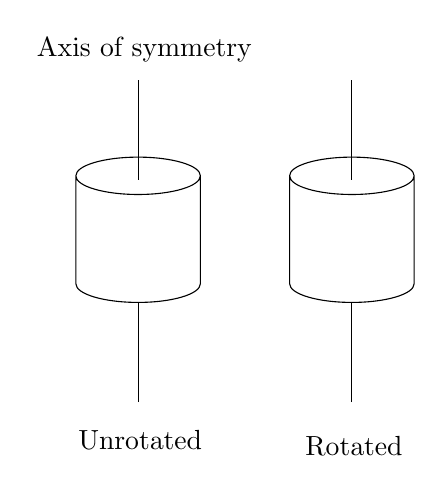
\begin{tikzpicture}[x=0.75pt,y=0.75pt,yscale=-1,xscale=1]
%uncomment if require: \path (0,300); %set diagram left start at 0, and has height of 300

%Shape: Can [id:dp6111663527038986] 
\draw   (154,122) -- (154,174) .. controls (154,178.97) and (140.57,183) .. (124,183) .. controls (107.43,183) and (94,178.97) .. (94,174) -- (94,122) .. controls (94,117.03) and (107.43,113) .. (124,113) .. controls (140.57,113) and (154,117.03) .. (154,122) .. controls (154,126.97) and (140.57,131) .. (124,131) .. controls (107.43,131) and (94,126.97) .. (94,122) ;
%Straight Lines [id:da6016989853853066] 
\draw    (124,124) -- (124,76) ;
%Straight Lines [id:da7742642520386162] 
\draw    (124,231) -- (124,183) ;
%Shape: Can [id:dp6333770541501842] 
\draw   (257,122) -- (257,174) .. controls (257,178.97) and (243.57,183) .. (227,183) .. controls (210.43,183) and (197,178.97) .. (197,174) -- (197,122) .. controls (197,117.03) and (210.43,113) .. (227,113) .. controls (243.57,113) and (257,117.03) .. (257,122) .. controls (257,126.97) and (243.57,131) .. (227,131) .. controls (210.43,131) and (197,126.97) .. (197,122) ;
%Straight Lines [id:da2230680788551479] 
\draw    (227,124) -- (227,76) ;
%Straight Lines [id:da2565843946616415] 
\draw    (227,231) -- (227,183) ;

% Text Node
\draw (125,249) node   [align=left] {Unrotated};
% Text Node
\draw (228,252) node   [align=left] {Rotated};
% Text Node
\draw (127,61) node   [align=left] {Axis of symmetry};


\end{tikzpicture}
    \caption{Symmetry of a cylinder}
    \label{fig:cylinder-rot}
\end{figure}
Mathematically, when we change our position of observation, it is equivalent to using a new, different reference frame and coordinate system, oriented differently from, and/or displaced relative to, the original. So a transformation can be viewed simply as a change of coordinate system, and this is often represented as a shifting from unprimed to primed coordinates. In QFT, \textbf{we will focus on passive transformation interpretation.}

\begin{example}
Consider the function 
\begin{equation}
g\left(x^{1}, x^{2}\right)=\left(x^{2}\right)^{2}
\end{equation}
if we have the following rorational transformation as
$$
\left[\begin{array}{l}
{x^{\prime 1}} \\
{x^{\prime 2}}
\end{array}\right]=\underbrace{\left[\begin{array}{cc}
{\cos \theta} & {\sin \theta} \\
{-\sin \theta} & {\cos \theta}
\end{array}\right]}_T\left[\begin{array}{l}
{x^{1}} \\
{x^{2}}
\end{array}\right]
\quad
\left[\begin{array}{l}
{x^{1}} \\
{x^{2}}
\end{array}\right]=\underbrace{\left[\begin{array}{ll}
{\cos \theta} & {-\sin \theta} \\
{\sin \theta} & {\cos \theta}
\end{array}\right]}_{T^{-1}=T^T}\left[\begin{array}{l}
{x^{\prime1}} \\
{x^{\prime2}}
\end{array}\right]
$$
we can express the function in the primed coordinate as:
$$
g=\left(x^{2}\right)^{2}=\left(x^{\prime 1} \sin \theta+x^{\prime 2} \cos \theta\right)^{2}=\left(x^{\prime 1}\right)^{2} \sin ^{2} \theta+\left(x^{\prime 2}\right)^{2} \cos ^{2} \theta+2 x^{\prime 1} x^{\prime 2} \sin \theta \cos \theta \neq\left(x^{\prime 2}\right)^{2}
$$
The transformed form of $g,$ represented by $g^{\prime}$, has the same value at the same physical point, but it is not the same form in terms of the primed coordinates as $g$ was in terms of the unprimed coordinates. But $f^{\prime},$ the transformed form of $f,$ did have the same form in terms of both sets of coordinates, and thus, we dropped the prime on $f$ on the RHS.

In spite of its non-symmetry under rotation, $g$ is symmetric under a different kind of Fransfort of the firc-symment ander founding $f$ the bynaced relative to the first along transformation, the translation to a coordinate system which is displaced relative to the first along the $x^{1}$ axis, i.e., $x^{1} \rightarrow x^{1}=x^{1}+$ constant $,$ or
$$
\left[\begin{array}{l}
{x^{\prime 1}} \\
{x^{\prime 2}}
\end{array}\right]=\left[\begin{array}{l}
{x^{1}} \\
{x^{2}}
\end{array}\right]+\left[\begin{array}{l}
{K} \\
{0}
\end{array}\right] \quad K=\text { constant }
$$
Substitution yields $g^{\prime}$ have the same form.
\end{example}
\begin{qt}
    From the example above, we can deduce the general rule that if a coordinate is missing in a given function, that function is invariant under a transformation solely in the direction of that coordinate (and also under multiplication of the coordiante by a constant).
\end{qt}
\textbf{\redp{So under any transformation of coordinate axes, the value at a physical point of every possible scalar function is invariant.}}
\subsection{Scalar are invariant, vectors are covariant}
\textbf{The scalar value at the point ( equal to the length of the position vector at that point) is the same in both systems, but the coordinate values are not.} For a 2D position vector in physical space, we have
$$
|x|=\left|x^{i}\right|=\sqrt{\left(x^{1}\right)^{2}+\left(x^{2}\right)^{2}}=\sqrt{\left(x^{\prime1}\right)^{2}+\left(x^{\prime2}\right)^{2}}=\left|x^{\prime i}\right|
$$
It is generally true of every vector $\mathbf{v},$ not just the position vector shown here, that its physical, measurable length (a scalar value) remains unchanged under any coordinate transformation, but its component values change. This is called covariance. Scalar values are invariant under coordinate transformation; vector components are \textbf{covariant}.
\begin{qt}
    General rule: if a function $h$ is not a function of the $j$th coordinate $x^j$, then h is symmetric under the transformation $x^{j} \rightarrow x^{j}+$ constant.
\end{qt}
\section{Symmetry in Classical Mechanics}
Recall that a Galilean transformation is
$$
\left[\begin{array}{c}
{x^{1}} \\
{x^{2}} \\
{x^{3}}
\end{array}\right] \rightarrow\left[\begin{array}{c}
{x^{11}} \\
{x^{\prime 2}} \\
{x^{3}}
\end{array}\right]=\left[\begin{array}{c}
{x^{1}-v^{1} t} \\
{x^{2}-v^{2} t} \\
{x^{3}-v^{3} t}
\end{array}\right]
$$
Newtonian mechanics is invariant under the Galilean transformation. But \textbf{Maxwell's eqs are not invariant under Galilean transformation. Instead, it is invariant under Lorentz transformation}
\begin{qt}
    \begin{equation}
\left[\begin{array}{c}
{x^{0}} \\
{x^{1}} \\
{x^{2}} \\
{x^{3}}
\end{array}\right] \rightarrow\left[\begin{array}{c}
{x^{\prime 0}} \\
{x^{\prime 1}} \\
{x^{\prime 2}} \\
{x^{\prime 3}}
\end{array}\right]=\left[\begin{array}{c}
{\gamma\left(x^{0}-\frac{v}{c} x^{1}\right)} \\
{\gamma\left(x^{1}-\frac{v}{c} x^{0}\right)} \\
{x^{2}} \\
{x^{3}}
\end{array}\right]=\underbrace{\left[\begin{array}{cccc}
{\gamma} & {-\gamma \frac{v}{c}} & {0} & {0} \\
{-\gamma \frac{v}{c}} & {\gamma} & {0} & {0} \\
{0} & {0} & {1} & {0} \\
{0} & {0} & {0} & {1}
\end{array}\right]}_{\Lambda}\left[\begin{array}{c}
{x^{0}} \\
{x^{1}} \\
{x^{2}} \\
{x^{3}}
\end{array}\right]
\label{lorentz-trans}
\end{equation}
where
$$
\gamma=\frac{1}{\sqrt{1-\frac{v^{2}}{c^{2}}}} \quad v=v^{1}
$$
\end{qt}
The index notation for Lorentz transformations is 
\begin{qt}
    \begin{equation}
x^{\prime \mu}=\Lambda^{\mu}{}_{v} x^{v} \quad V^{\prime \mu}\left(x^{\prime \alpha}\right)=\Lambda^{\mu}{}_{v} V^{v}\left(x^{\alpha}\right) \quad T^{\prime \mu v}\left(x^{\prime \alpha}\right)=\Lambda^{\mu}{}_{\delta} \Lambda^{v}{}_{\gamma} T^{\delta \gamma}\left(x^{\alpha}\right)
\end{equation}
Note that $\Lambda^{-1},$ the inverse of $\Lambda,$ can be obtained by taking $\mathbf{v} \rightarrow-\mathbf{v}$ since each coordinate system seems to be going in the opposite direction with respect to the other. $\Lambda^{-1}$ will transform $x^{\prime \mu}$ back into $x^{\mu}$.
\end{qt}
\bluep{Recall that the length of a vector in 3D is unchanged under a coordinate system transformation, 1.e., the length 1s a scalar and thus invariant. The same thing is true in 4D for four-vectors.}
$$
w_{\mu} w^{\mu}=w_{0} w^{0}+w_{1} w^{1}+w_{2} w^{2}+w_{3} w^{3}=w^{0} w^{0}-w^{1} w^{1}-w^{2} w^{2}-w^{3} w^{3}=\text { scalar invariant }
$$
\textbf{and that this is the same for any observer in any inertial coordinate system. This applies to any
vector, be it a position vector like $x^{\mu},$ the differential of position $d x^{\mu},$ the four-velocity $u^{\mu}$, the four potential $A^{\mu}$, the partial derivative $\partial^{\mu}$, or any other}.For instance,
$$
\frac{\partial}{\partial x^{\mu}} \frac{\partial}{\partial x_{\mu}}=\partial_{\mu} \partial^{\mu}=\frac{\partial}{\partial x^{0}} \frac{\partial}{\partial x^{0}}-\frac{\partial}{\partial x^{1}} \frac{\partial}{\partial x^{1}}-\frac{\partial}{\partial x^{2}} \frac{\partial}{\partial x^{2}}-\frac{\partial}{\partial x^{3}} \frac{\partial}{\partial x^{3}}=\text { scalar invariant derivative, }
$$
So if X represents a quantity, we have
$$
\frac{\partial}{\partial x^{\mu}} \frac{\partial}{\partial x_{\mu}}=\frac{\partial}{\partial x^{\prime \mu}} \frac{\partial}{\partial x_{\mu}^{\prime}} \rightarrow \frac{\partial}{\partial x^{\mu}} \frac{\partial}{\partial x_{\mu}} X=\frac{\partial}{\partial x^{\prime\mu}} \frac{\partial}{\partial x_{\mu}^{\prime}} X
$$
\subsection{Poincare transformation}
The most general transformation we could have in spacetime would comprise 1) a 4D translation(translating our coordinate axes in space, time, or both), 2) a rotation in space, and 3) a Lorentz transformation to a frame with different relative velocity. (We ignore reflection.)

The rotation in 3D is the same. It does allow us to rotate our 3D axes, however, so that the relative velocity between our original and transformed systems is along the $x^1$ axes of both. \textbf{This lets us use the Lorentz transformation in its simplest form (\ref{lorentz-trans})}. With this form we state the general transformation between coordinate systems, know as \redp{\textbf{Poincare transformation}} as
\begin{equation}
x^{\mu}=\Lambda_{\nu}^{\mu}\left(x^{\nu}+a^{\nu}\right) \quad a^{\nu}=\mathrm{constant} \text { four vector }
\label{poincare-trans}
\end{equation}

\subsection{Other kinds of symmetry}
Consider the Euler-Lagrange equation for a particle in Newtonian mechanics
$$
\frac{d}{d t}\left(\frac{\partial L}{\partial \dot{x}^{i}}\right)-\frac{\partial L}{\partial x^{i}}=0 \quad L=T-V \quad p_{i}=\frac{\partial L}{\partial \dot{x}^{i}}
$$
If the Lagrangian $L$ is not an explicit function of the spatial coordinate $x^i,$ then $\partial L / \partial x^{i}=0$ on the LHS above. Thus, the time derivative of $p_{i}$ is zero.
$$
\frac{d}{d t}\left(\frac{\partial L}{\partial \dot{x}^{i}}\right)=\frac{d p_{i}}{d t}=0 \quad \text { with } \frac{\partial L}{\partial x^{i}}=0 \quad \text { when } \quad L \neq L\left(x^{i}\right)
$$
Hence $p^i$ is constant and thus, conserved. This makes sense since the only source for spatial dependence in $L$ is the potential energy $V$. If we have no $V$ dependence on $x^i$, then there is no force in the $x^i$ direction, and momentum $p_i$ is constant.\textbf{Note this means the Lagrangian is symmtric.}

\redp{If the Lagrangian is symmetric in a coordinate, then the conjugate momentum for that coordiante is conserved.}

\section{Transformations in QFT}
\subsection{Spinor transformation}
For spinor, we seek a matrix which is four by four in spinor space and which represents what ha~pens to a spmor under a Lorentz transformation and/or a rotation of coordinates. That is, we seek D in
\begin{equation}
\psi^{\prime}\left(x^{\prime \mu}\right)=D \psi\left(x^{\mu}\right) \quad \frac{\text { with spinor indices }}{\text { written out }} \quad \psi_{\alpha}^{\prime}\left(x^{\prime \mu}\right)=D_{\alpha \beta} \psi_{\beta}\left(x^{\mu}\right)
\end{equation}
The spinor transformation under Lorentz and rotation transformation is
\begin{equation}
D=e^{-i(\mathbf{L} \mathbf{\Theta}+\mathbf{M} \mathbf{Q})} \quad L^{k}=-\frac{i}{2} \varepsilon_{i j}^{k} \gamma^{i} \gamma^{j}, \quad \Theta^{k}=\left(\theta^{1}, \theta^{2}, \theta^{3}\right), M^{k}=\frac{i}{2} \gamma^{0} \gamma^{k}, Q^{k}=\left(v^{1}, v^{2}, v^{3}\right)
\end{equation}
where $\Theta^{k}$ represents rotation angles of the primed system with respect to the unprimed system; $Q^k$ is a three vector of the boost velocities; and $\epsilon_{ij}{}^{k}$ is zero unless $i,j,k$ are all different, 1 if $ijk=123,231,312$, and -1 for the others.

Note that in formal mathematical language, the set of all possible Lorentz transformations (all possible v) is known as the Lorentz group. When the Lorentz group acts on the coordinate system, it changes what our spinors look like in the new system and this change is represented by $D$. So, \textbf{$D$ is called a representation of the Lorentz group.} It "represents" that group in spinor space.
\begin{qt}
    $\bar{\psi} \psi=$ world scalar $\quad \bar{\psi} \gamma^{\mu} \psi=$ transforms like four vector.
\end{qt}
\section{Lorentz Symmetry of the Lagrangian Density}
Lagrangian Density is symmetric under Lorentz transformation. We conclude this because of Einstein's postulate that the laws of nature (the field equation here) is invariant in form under Lorentz transformation. The Euler-Lagrange equation for fields, which is another form of the field equation, is a law of nature and must, therefore be invariant in form as well.

\section{Noether's Theorem}
There are other ways the Lagrangian density can be symmetric, for example
\begin{equation}
\phi \rightarrow \phi^{\prime}=\phi e^{-i \alpha}
\label{phase-trans}
\end{equation}
and for free scalar field, we have
$$
\mathcal{L}_{0}^{0}=\partial_{v} \underbrace{\phi^{r+} e^{-i \alpha}}_{\phi^{\dagger}} \partial^{v} \underbrace{\phi^{\prime} e^{i a}}_{\phi}-\mu^{2} \underbrace{\phi^{\prime} e^{-i \alpha}}_{\phi^{\dagger}} \underbrace{\phi^{\prime} e^{i \alpha}}_{\phi}=\mathcal{L}_{0}^{0}\left(\phi^{\prime\dagger}, \phi^{\prime}\right)
$$
\subsection{Internal and external symmetries}
Poincaré transformations (Lorentz plus $4 \mathrm{D}$ translation) and $3 \mathrm{D}$ rotations involve changes $\mathrm{t}$ to physical coordinates $x^{\mu}$ of our external world and are called \textbf{external transformations}.

Transformation like (\ref{phase-trans}) have nothing to do with $x^{\mu}$, but instead function in hidden spaces, behind the scene, like Hilbert or Fock space. They are called \textbf{internal transformation}.
\begin{qt}
   Noether's theorem in words: \textbf{ A symmetry in the Lagrangian density implies an associated quantity is conserved.}
   
   Mathematically:If the Lagrangian density $\mathcal{L}\left(\phi^{r}, \phi^{r}, \mu\right)$ is symmetric in form with respect to a transformation in $\phi^{r}$ which is a function of parameter $\alpha$,i.e., $\phi^{r}\left(x^{\mu}\right) \rightarrow \phi^{r}\left(x^{\mu}, \alpha\right)$ then the four current (using $\left.\phi^{r}\left(x^{\mu}, \alpha\right)\right)$
   \begin{equation}
j^{\mu}\left(\phi^{r}, \phi_{, \nu}^{r}\right)=\frac{\partial \mathcal{L}}{\partial \phi_{, \mu}^{r}} \frac{\partial \phi^{r}}{\partial \alpha} \quad(\text { sum on } r)
\end{equation}
bas zero four-divergence,$\partial_{\mu} j^{\mu}=0$. Thus, its zeroth component $j^0$ integrated over all the space is conserved, as is $q j^{0}$ integrated over all space, where $q$ is a constant.
\end{qt}
\subsection{Apply Noether's theorem to free scalar field}
$$
\frac{\partial \mathcal{L}_{0}^{0}}{\partial \phi_{\mu}}=\frac{\partial}{\partial \phi_{, \mu}}\left(\phi_{, \nu}^{\dagger} \phi^{\nu}-\mu^{2} \phi^{\dagger} \phi\right)=\frac{\partial}{\partial \phi_{\mu}}\left(\phi_{, \mu}^{\dagger} \phi^{\nu}\right)
=\frac{\partial \phi_{, \nu}^{\dagger}}{\partial \phi_{\mu}} \phi^{,\nu}+\phi_{, \nu}^{\dagger} \frac{\partial \phi^{,\nu}}{\partial \phi_{,\mu}}=\phi_{, \nu}^{\dagger} g^{\nu \mu}=\phi^{\dagger, \mu}
$$
$$
\frac{\partial \mathcal{L}_{0}^{0}}{\partial \phi^{\dagger}, \mu}=\frac{\partial}{\partial \phi^{\dagger}, \mu}\left(\phi_{, \nu}^{\dagger} \phi^{\nu}-\mu^{2} \phi^{\dagger} \phi\right)=\frac{\partial}{\partial \phi^{\dagger}}\left(\phi^{\dagger}, \phi^{,\nu}\right)=\frac{\partial \phi^{\dagger}_{, \nu}}{\partial \phi^{\dagger}_{, \mu}} \phi^{,\nu}=\delta_{v}^{\mu} \phi^{, v}=\phi^{,\mu}
$$
and
$$
\begin{array}{l}
{\frac{\partial \phi\left(x^{\eta}, \alpha\right)}{\partial \alpha}=\frac{\partial}{\partial \alpha} \phi\left(x^{\eta}\right) e^{-i \alpha}=-i \phi\left(x^{\eta}\right) e^{-i \alpha}} \\
{\frac{\partial \phi^{\dagger}\left(x^{\eta}, \alpha\right)}{\partial \alpha}=\frac{\partial}{\partial \alpha} \phi^{\dagger}\left(x^{\eta}\right) e^{i \alpha}=i \phi^{\dagger}\left(x^{\eta}\right) e^{i \alpha}}
\end{array}
$$
Using the relation above, we have
$$
j^{\mu}\left(\phi^{r}, \phi^{r}_{,v}\right)=i\left(\phi^{,\mu}\left(x^{\eta}\right) \phi^{\dagger}\left(x^{\eta}\right)-\phi^{\dagger, \mu}\left(x^{\eta}\right) \phi\left(x^{\eta}\right)\right)
$$
This is identical to the scalar four-current.\redp{The expectation value ( expected measurement) of a conserved operator is conserved. If the state measured is in an eigenstate, any measurement at any time will yield the same eigenvalue}.
\section{Symmetry, Gauges, and Gauge theory}
\begin{itemize}
    \item \textbf{Gauge invariance }(or gauge symmetry) is the property of a field theory in which different configurations of the underlying fundamental, but unobservable, field(s) result in identical observable properties.
    \item the unobservable field, often a potential field, is called the\textbf{ gauge field}.
    \item A gauge transformation changes the gauge field from one configuration to another. \redp{Each different configuration of the gauge field is a different gauge.}
    \item A theory have gauge invariance (symmetry) is called a gauge theory.
\end{itemize}
\redp{\textbf{We can also say that a gauge theory is a type of field theory in which the Lagrangian ( density) is invariant under a continuous (not discrete) transformation.}}
\section{A Solved Exercises}
\textbf{Problem 14.} Show that the total (not density) 3-momentum $k^{i}$ for free scalars is conserved. Use our knowledge that the conjugate momentum for $x^{i}$ is $k_{i}$, the total (not density) 3 -momentum (expressed in covariant components), and it is conserved if $L$ is symmetric (invariant) under the coordinate translation transformation $x^{t} \rightarrow x^{1}=x^{t},$ where $\alpha^{t}$ is a constant $3 \square$ vector. Then, show the same result via commutation of the three-momentum operator.

\textbf{Solution}
The Lagrangian density is $\mathcal{L}_{0}^{0}=\phi_{, \mu}^{\dagger} \phi^{\mu}-\mu^{2} \phi^{\dagger} \phi .$ We must integrate this over all volume to get the total Lagrangian $L$. If $k_{i}$ is conserved, then of course, so is $k^{i}$. So, we need to show $L$ is invariant under $x^{i} \rightarrow x^{i}=x^{i}+\alpha^{i}$
$$
\phi=\sum_{\mathbf{k}} \frac{1}{\sqrt{2 V a_{\mathbf{k}}}}\left(a(\mathbf{k}) e^{-i k_{\mu} x^{\mu}}+b^{\dagger}(\mathbf{k}) e^{i k_{\mu} x^{\mu}}\right) \quad \phi^{\dagger}=\sum_{\mathbf{k}} \frac{1}{\sqrt{2 V a_{k}}}\left(b(\mathbf{k}) e^{-i k_{\mu} x^{\mu}}+a^{\dagger}(\mathbf{k}) e^{i k_{\mu} x^{\mu}}\right)
$$
$$
\begin{array}{l}
{\phi_{s}, \mu=\sum_{\mathbf{k}} \frac{i k_{\mu}}{\sqrt{2 V \omega_{\mathbf{k}}}}\left(-a(\mathbf{k}) e^{-i k_{\mu} x^{\mu}}+b^{\dagger}(\mathbf{k}) e^{i k_{\mu} x^{\mu}}\right)} \\
{\phi^{, \mu}=\sum_{\mathbf{k}} \frac{i k^{\mu}}{\sqrt{2 V a_{k}}}\left(-a(\mathbf{k}) e^{-i k_{\mu} x^{\mu}}+b^{\dagger}(\mathbf{k}) e^{i k_{\mu} x^{\mu}}\right)}
\end{array}
$$
$$
\begin{aligned}
\phi^{\dagger}_{z \mu} \phi^{z}=\sum_{\mathbf{k}} \sum_{\mathbf{k}^{*}} \frac{-1}{2 V} \frac{k_{\mu} k^{* \mu}}{\sqrt{\omega_{\mathbf{k}} \omega_{\mathbf{k}^{*}}}}\left(b(\mathbf{k}) a\left(\mathbf{k}^{*}\right) e^{-i k_{A} x^{\mu}} e^{-i k_{A}^{*} x^{\mu}}-b(\mathbf{k}) b^{\dagger}\left(\mathbf{k}^{*}\right) e^{-i k_{\mu} x^{\mu}} e^{i k_{\mu} x^{\mu}}\right.\\
-a^{\dagger}(\mathbf{k}) a\left(\mathbf{k}^{*}\right) e^{i k_{\mu} x^{\mu}} e^{-i k_{\mu} x^{\mu}}+a^{\dagger}(\mathbf{k}) b^{\dagger}\left(\mathbf{k}^{*}\right) e^{i k_{\mu} x^{\mu}} e^{i k_{\mu} x^{\mu}}
\end{aligned}
$$
For $k_{i}=-k^*_i$, we have $$
\left.k_{\mu} k^{* \mu}=\omega_{\mathbf{k}}^{2}+k_{i} k^{*i}=\omega_{\mathbf{k}}^{2}+k_{i}\left(-k^{i}\right)=\omega_{\mathbf{k}}^{2}+k_{i} k_{i}=k_{\mu} k_{\mu}\right.
$$
$$
\int \phi^{\dagger}_{,\mu} \phi^{, \mu} d V=\sum_{k} \frac{-1}{2 \omega_{k}}\left(\begin{array}{c}
{k_{\mu} k_{\mu} e^{-i 2 \omega_{k} t} b(\mathbf{k}) a(-\mathbf{k})-k_{\mu} k^{\mu} b(\mathbf{k}) b^{\dagger}(\mathbf{k})} \\
{-k_{\mu} k^{\mu} a^{\dagger}(\mathbf{k}) a(\mathbf{k})+k_{\mu} k_{\mu} e^{i 2 \omega_{k} t} a^{\dagger}(\mathbf{k}) b^{\dagger}(-\mathbf{k})}
\end{array}\right)
$$
Similarly,
$$
\int \mu^{2} \phi^{\dagger} \phi d V=-\sum_{\mathbf{k}} \frac{\mu^{2}}{2 \omega_{\mathbf{k}}}\left(e^{-i 2 \omega_{\mathbf{k}} t} b(\mathbf{k}) a(-\mathbf{k})+b(\mathbf{k}) b^{\dagger}(\mathbf{k})+a^{\dagger}(\mathbf{k}) a(\mathbf{k})+e^{i 2 \omega_{\mathbf{k}} t} a^{\dagger}(\mathbf{k}) b^{\dagger}(-\mathbf{k})\right)
$$
It is easy to show that, after the transformation the forms of $\int \mu^{2} \phi^{\dagger} \phi d V$ and $\int \phi^{\dagger}_{,\mu} \phi^{, \mu} d V$ will not change, so L is symmetric in some coordinate, then the conjugate momentum of that coordinate is conserved. $k_{i}$, the particle(s) 3 -momentum is the conjugate momentum of $x^{i} .$ Thus, $k_{i}$, is conserved.

Also
$$
H=\sum_{\mathbf{k}} \omega_{\mathbf{k}}\left(N_{a}(\mathbf{k})+N_{b}(\mathbf{k})\right) \quad \mathbf{P}=\sum_{\mathbf{k}} \mathbf{k}\left(N_{a}(\mathbf{k})+N_{b}(\mathbf{k})\right) \rightarrow[H, \mathbf{P}]=0 \quad\left(\begin{array}{ll}
{\text { because all number }} \\
{\text { operators commute }}
\end{array}\right)
$$
Thus $\mathbf{P}$ is conserved for the free Hamiltonian.
\end{document}
